\section{Introducere}
În anii recenți rețelele convoluționale [\ref{fig:cnn}] s-au dovedit foarte utile în rezolvarea problemelor care conțin imagini. Spre deosebire de rețelele neurale simple, acestea păstrează spațialitatea imaginii și de aceea se comportă mai bine. În anumite sarcini, precum recunoașterea de obiecte dintr-o poza, rețele neurale convoluționale aproape au atins performanța omului în distingerea obiectelor. Pentru o mai bună înțelegere despre cum funcționează aceste rețele voi prezenta un exemplu. \cite{coursera_convnets}\cite{matthew2013} Alegem un neuron dintr-un anumit layer al rețelei și vedem cum arată porțiunea din imagine pentru care activarea acestui neuron este maximă. În imaginile [\ref{fig:cnn_layer1}, \ref{fig:cnn_layer2}, \ref{fig:cnn_layer3}, \ref{fig:cnn_layer4}, \ref{fig:cnn_layer5}], care au fost luate din articolul lui Matthew D. Zeiler, Visualizing and Understanding Convolutional Networks apărut în anul 2013 \cite{matthew2013}, pentru fiecare layer în parte, au fost aleși diferiți neuroni din layer-ul respectiv, iar pentru fiecare neuron, au fost alese noua imagini care maximizează activarea neuronului și afișată porțiunea pe care neuronul respectiv o vede din poza întreagă.
\begin{figure}[h]
	\centering
	\begin{subfigure}[b]{0.4\textwidth}
		\centering
        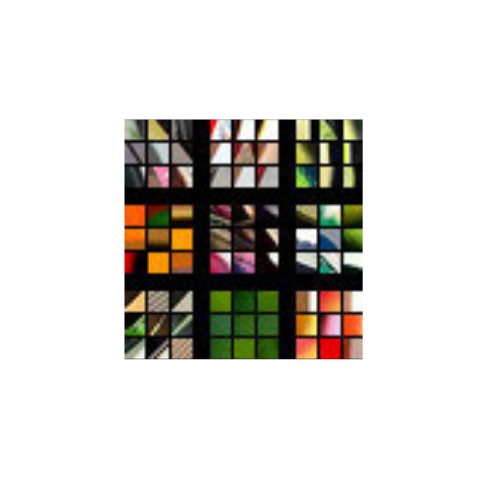
\includegraphics[height=8cm, width=\textwidth]{cnn_layer1}
        \caption{Layer 1. După cum se poate observa în această poză, neuronii din primul layer tind să se activeze la caracteristici precum linii sau anumite nuanțe de culoare. De exemplu, în colțul din stânga sus neuronul respectiv a avut o activare mare la porțiunile din imagine care conțin linii oblice. Pe când, la zona din mijloc de pe ultimul rând, un alt neuron s-a activat când în porțiunea pe care acesta o vede erau diferite nuanțe de verde.}
        \label{fig:cnn_layer1}
	\end{subfigure}
    \hfill
    \begin{subfigure}[b]{0.4\textwidth}
		\centering
        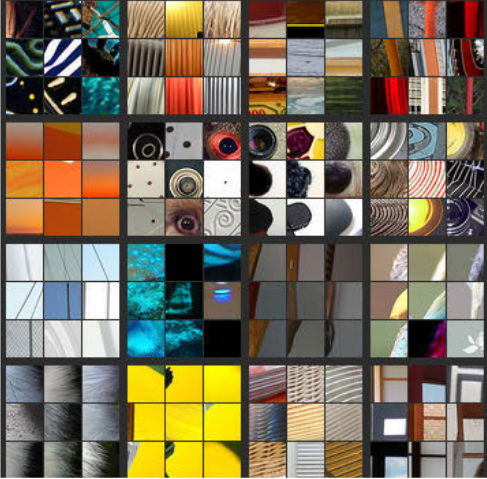
\includegraphics[height=8cm, width=\textwidth]{cnn_layer2}
        \caption{Layer 2. Neuronii din acest layer s-au activat la caracteristici mai complexe decât cele la care s-au activat neuronii din primul layer. Se poate observa de exemplu în poza a doua de pe primul rând că neuronul respectiv s-a activat când a văzut un fel de textură alcătuită din linii. În ultima poză de pe primul rând, neuronul respectiv se uită la acele porțiuni din imagine care conțin o linie verticală în centru.}
        \label{fig:cnn_layer2}
	\end{subfigure}
    \caption{Layer 1 și layer 2}
    \label{fig:cnn_layer1_2}
\end{figure}
\begin{figure}[h]
		\centering
        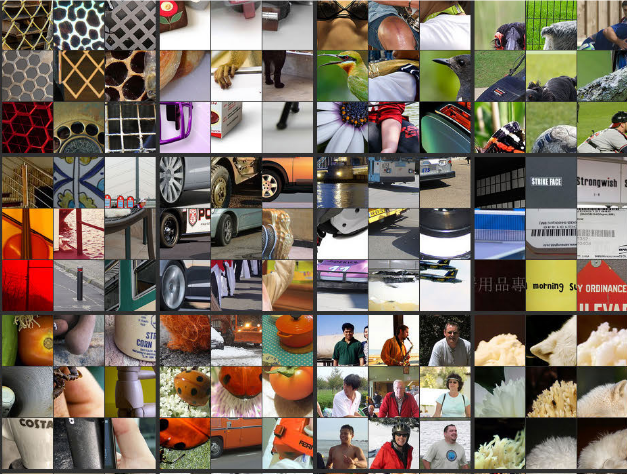
\includegraphics[height=8cm, width=\textwidth]{cnn_layer3}
        \caption{Layer 3. În acest layer de exemplu, în poza din colțul stânga sus, neuronul respectiv detectează un anumit fel de textură. În poza a treia de pe ultimul rând se observă că acel neuron se activează la oameni care stau într-o anumită poziție.}
        \label{fig:cnn_layer3}
\end{figure}
\begin{figure}[h]
	\centering
	\begin{subfigure}[b]{0.4\textwidth}
		\centering
        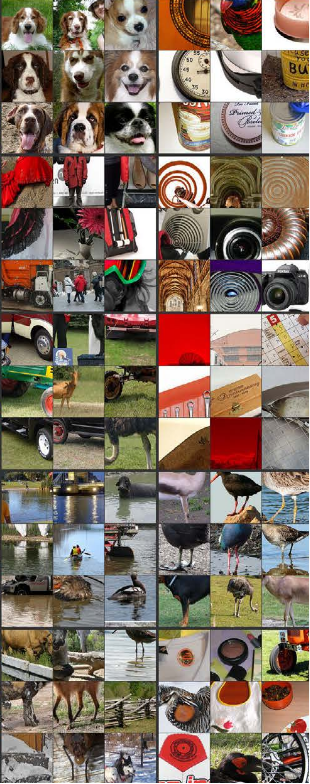
\includegraphics[height=11cm, width=\textwidth]{cnn_layer4}
        \caption{Layer 4. În acest layer de exemplu, în poza din colțul stânga sus se observă că neuronul respectiv a învățat să detecteze o anumită rasă de câini. Pe când neuronul din poza din dreapta de pe al patrulea rând se uită la picioare de animale.}
        \label{fig:cnn_layer4}
	\end{subfigure}
    \hfill
    \begin{subfigure}[b]{0.4\textwidth}
		\centering
        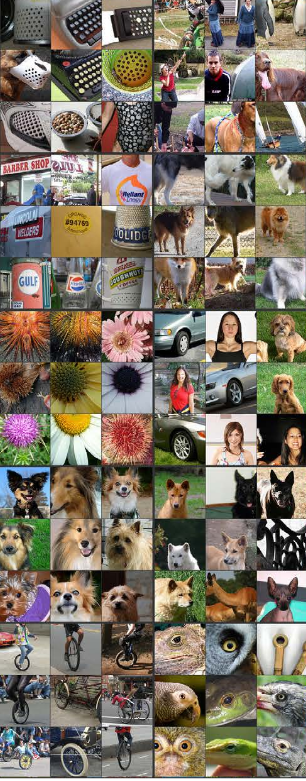
\includegraphics[height=11cm, width=\textwidth]{cnn_layer5}
        \caption{Layer 5. În acest layer de exemplu, în poza din stânga de pe ultimul rând se observă că neuronul respectiv a avut activarea maximă când în poză sunt roți subțiri. Pe când, tot pe acest rând, dar la poza din dreapta, neuronul respectiv se uită la ochi de animale.}
        \label{fig:cnn_layer5}
	\end{subfigure}
    \caption{Layer 4 și layer 5}
    \label{fig:cnn_layer4_5}
\end{figure}

O explicație pentru care caracteristicile la care se activează neuronii din layerele mai adânci sunt mai complexe este aceea că de-a lungul rețelei neurale, poza este micșorată și astfel neuronii văd o porțiune mai mare din imagine. De asemenea, neuronii din fiecare layer se uită la activările neuronilor din layerul precedent, și astfel combinând caracteristici simple se obțin caracteristici mai complexe.

\subsection{Generarea conținutului}
\label{ss:genc}
Din exemplul de mai sus, se observă că atunci când o rețea neurală convoluțională este antrenată să recunoască diferite obiecte dintr-o imagine, aceasta învață să se uite la caracteristici complexe din imagine și astfel este posibil ca având o poză inițializată cu zgomot aleator, o poză oarecare și o funcție de cost bazată pe cele două poze și pe activările neuronilor dintr-un anumit layer, să obținem din poza cu zgomot o poză asemănătoare cu cea pe care o dorim să o recreăm. \cite{mahendran2014} Astfel, bazându-ne pe această ideea putem genera o poză cu conținut asemănător cu cel al unei poze aleatoare alegând un singur layer.

În figura [\ref{fig:content_rec}] se poate observa mai bine ce am spus mai sus. Pe prima coloană se afla poza cu conținut pe care am dorit să o recreez, pe a doua coloană se află imaginea reconstruită, pornind de la o imagine inițializată cu zgomot, iar pe a treia coloană se află o parte din imaginea respectivă pentru a se vedea mai bine detaliile. Pentru poza de la $A$ am folosit activările din layerul \textit{conv1{\_}2}, pentru poza de la $B$ am ales layerul \textit{conv2{\_}2}, pentru poza de la $C$ am ales layerul \textit{conv3{\_}2}, pentru poza de la $D$ am ales layerul \textit{conv4{\_}2}, iar pentru poza de la $E$ am ales layerul \textit{conv5{\_}2}, peste toate aceste activări am aplicat ReLU. Se observă că dacă se generează poza folosind primele layere, atunci pixelii acesteia au aproape aceleași valori ca și pixelii din poza inițială, pe când dacă se generează poza folosind layere aflate mai departe în rețea se păstrează conținutul, dar pixelii sunt diferiți.

\begin{figure}[h]
	\centering
    \begin{subfigure}[b]{0.3\textwidth}
    	A
		\centering
        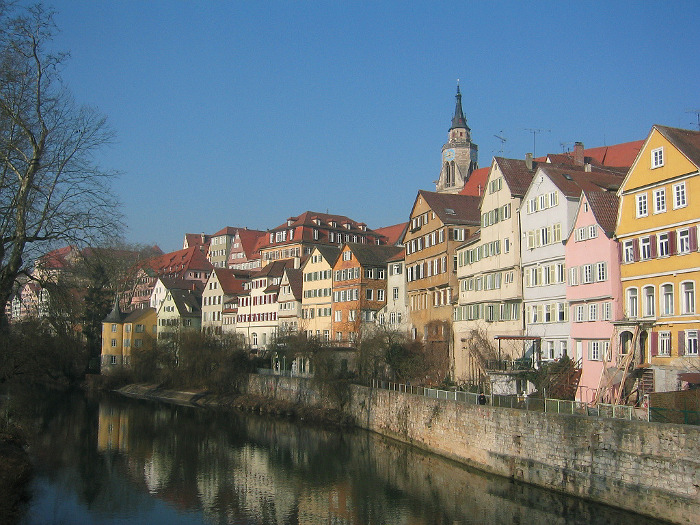
\includegraphics[height=4cm, width=0.9\textwidth]{content1}
        \label{fig:content}
	\end{subfigure}
    \hfill
    \begin{subfigure}[b]{0.3\textwidth}
		\centering
        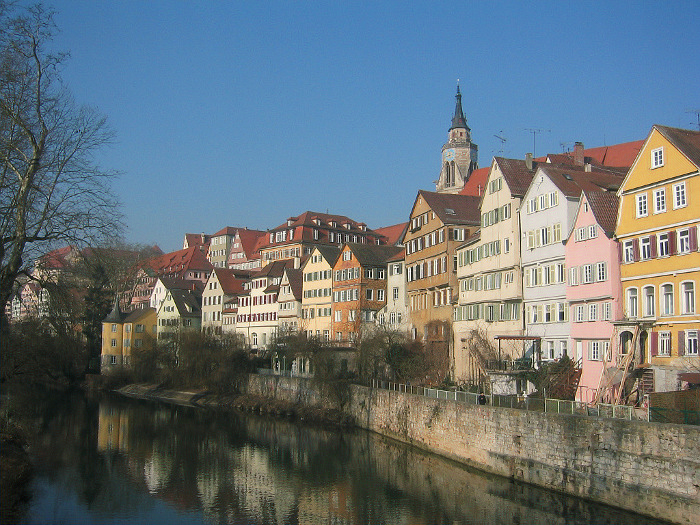
\includegraphics[height=4cm, width=0.9\textwidth]{content_relu1_2}
        \label{fig:content_relu1_2}
	\end{subfigure}
    \hfill
    \begin{subfigure}[b]{0.3\textwidth}
		\centering
        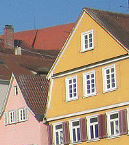
\includegraphics[height=4cm, width=0.9\textwidth]{content_relu1_2_crop}
        \label{fig:content_relu1_2_crop}
	\end{subfigure}
    \begin{subfigure}[b]{0.3\textwidth}
    	B
		\centering
        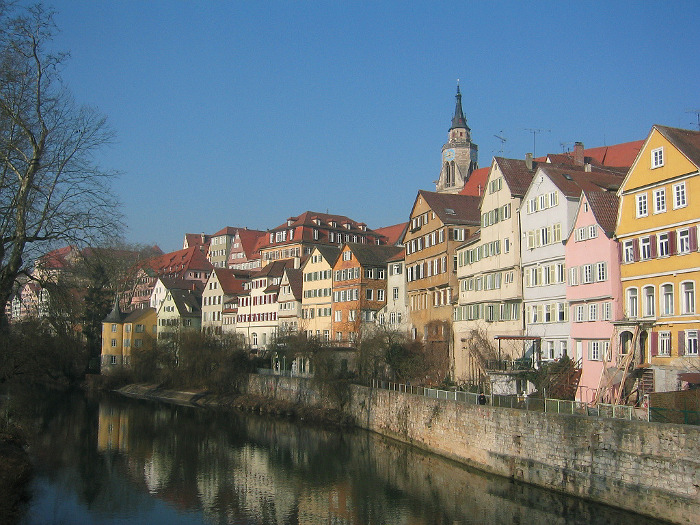
\includegraphics[height=4cm, width=0.9\textwidth]{content1}
        \label{fig:content}
	\end{subfigure}
    \hfill
    \begin{subfigure}[b]{0.3\textwidth}
		\centering
        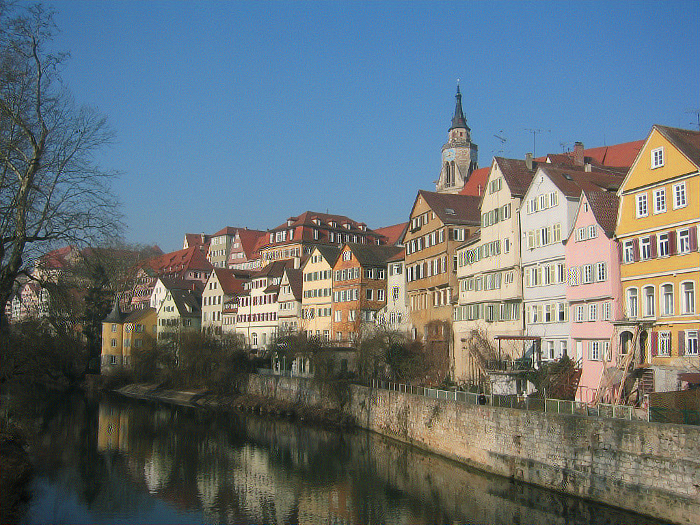
\includegraphics[height=4cm, width=0.9\textwidth]{content_relu2_2}
        \label{fig:content_relu2_2}
	\end{subfigure}
    \hfill
    \begin{subfigure}[b]{0.3\textwidth}
		\centering
        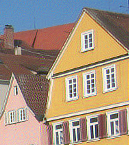
\includegraphics[height=4cm, width=0.9\textwidth]{content_relu2_2_crop}
        \label{fig:content_relu2_2_crop}
	\end{subfigure}
    \begin{subfigure}[b]{0.3\textwidth}
    	C
		\centering
        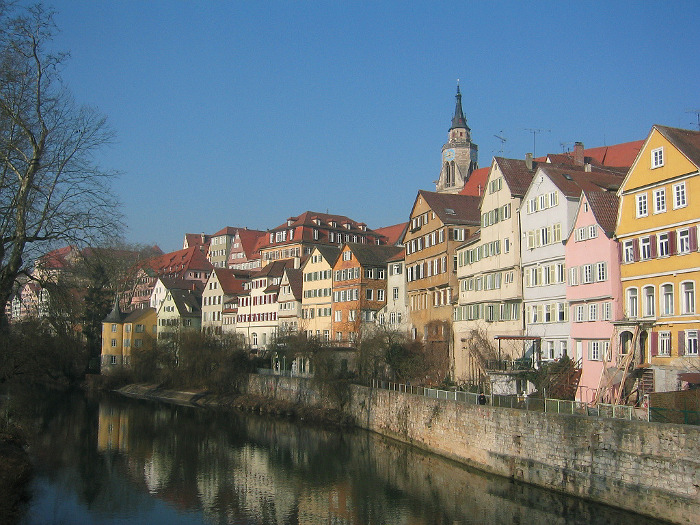
\includegraphics[height=4cm, width=0.9\textwidth]{content1}
        \label{fig:content}
	\end{subfigure}
    \hfill
    \begin{subfigure}[b]{0.3\textwidth}
		\centering
        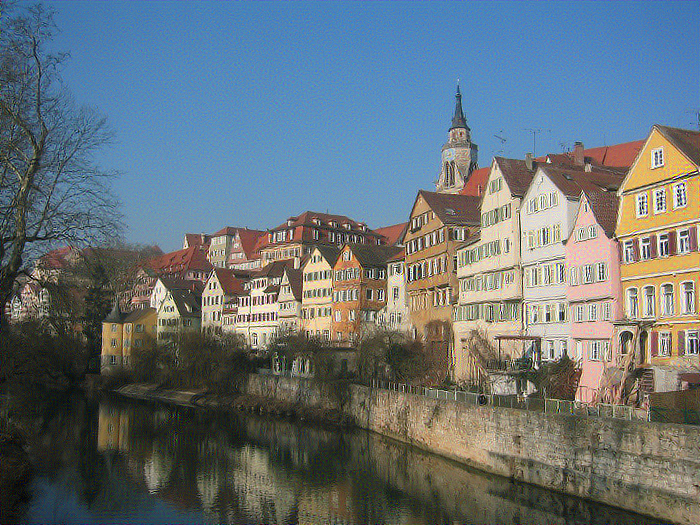
\includegraphics[height=4cm, width=0.9\textwidth]{content_relu3_2}
        \label{fig:content_relu3_2}
	\end{subfigure}
    \hfill
    \begin{subfigure}[b]{0.3\textwidth}
		\centering
        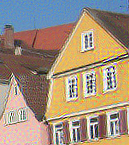
\includegraphics[height=4cm, width=0.9\textwidth]{content_relu3_2_crop}
        \label{fig:content_relu3_2_crop}
	\end{subfigure}
    \begin{subfigure}[b]{0.3\textwidth}
    	D
		\centering
        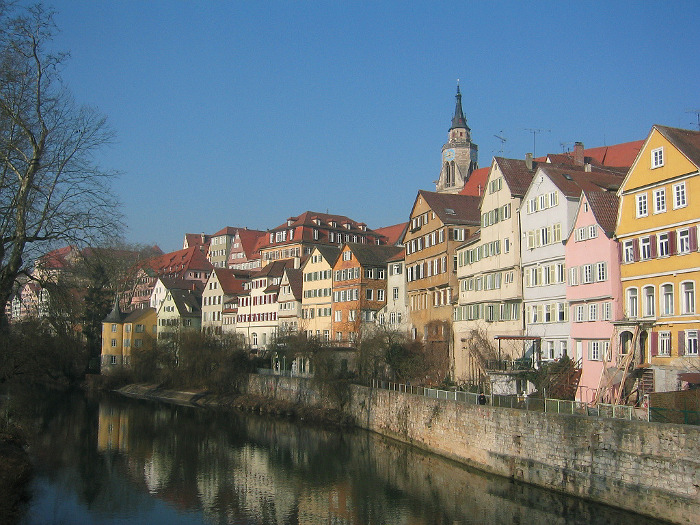
\includegraphics[height=4cm, width=0.9\textwidth]{content1}
        \label{fig:content}
	\end{subfigure}
    \hfill
    \begin{subfigure}[b]{0.3\textwidth}
		\centering
        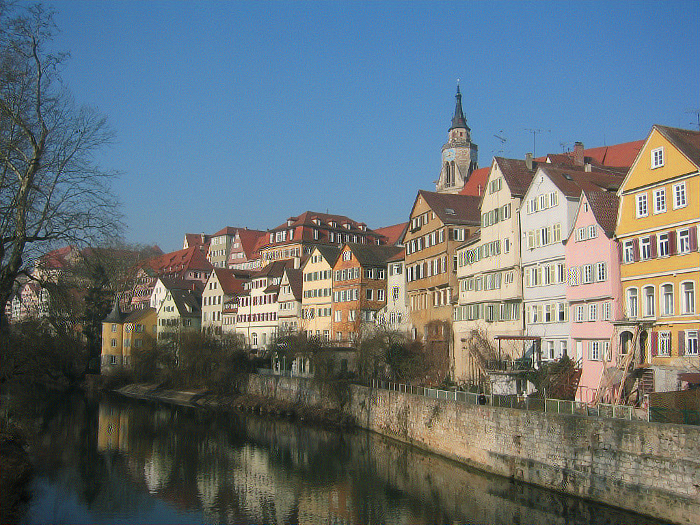
\includegraphics[height=4cm, width=0.9\textwidth]{content_relu2_2}
        \label{fig:content_relu4_2}
	\end{subfigure}
    \hfill
    \begin{subfigure}[b]{0.3\textwidth}
		\centering
        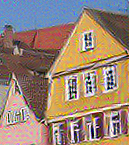
\includegraphics[height=4cm, width=0.9\textwidth]{content_relu4_2_crop}
        \label{fig:content_relu4_2_crop}
	\end{subfigure}
    \begin{subfigure}[b]{0.3\textwidth}
    	E
		\centering
        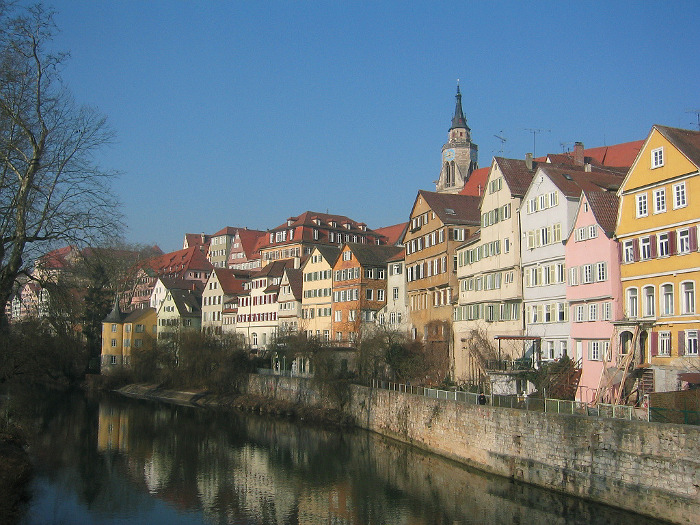
\includegraphics[height=4cm, width=0.9\textwidth]{content1}
        \label{fig:content}
	\end{subfigure}
    \hfill
    \begin{subfigure}[b]{0.3\textwidth}
		\centering
        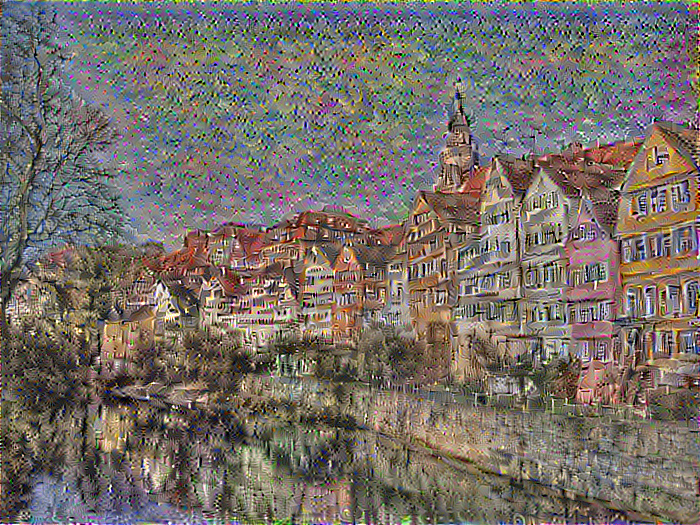
\includegraphics[height=4cm, width=0.9\textwidth]{content_relu5_2}
        \label{fig:content_relu5_2}
	\end{subfigure}
    \hfill
    \begin{subfigure}[b]{0.3\textwidth}
		\centering
        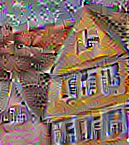
\includegraphics[height=4cm, width=0.9\textwidth]{content_relu5_2_crop}
        \label{fig:content_relu5_2_crop}
	\end{subfigure}
    \caption{Generarea conținutului}
    \label{fig:content_rec}
\end{figure}

\subsection{Generarea stilului}
\label{ss:gens}
După cum am spus, rețelele neurale convoluționale păstrează spațialitatea imaginii și o modelează cu ajutorul filtrelor aplicate asupra acesteia. Dacă atunci când optimizăm o poză cu zgomot, definim o funcție de cost care ține cont de corelația dintre filtrele pozei din unul sau mai multe layere, atunci se obține o textură alcătuită din elemente ale pozei de intrare, precum culoare, linii, diferite forme, etc. \cite{gatys_texture2015}

\begin{figure}[h]
	\centering
    \begin{subfigure}[b]{0.4\textwidth}
    	A
		\centering
        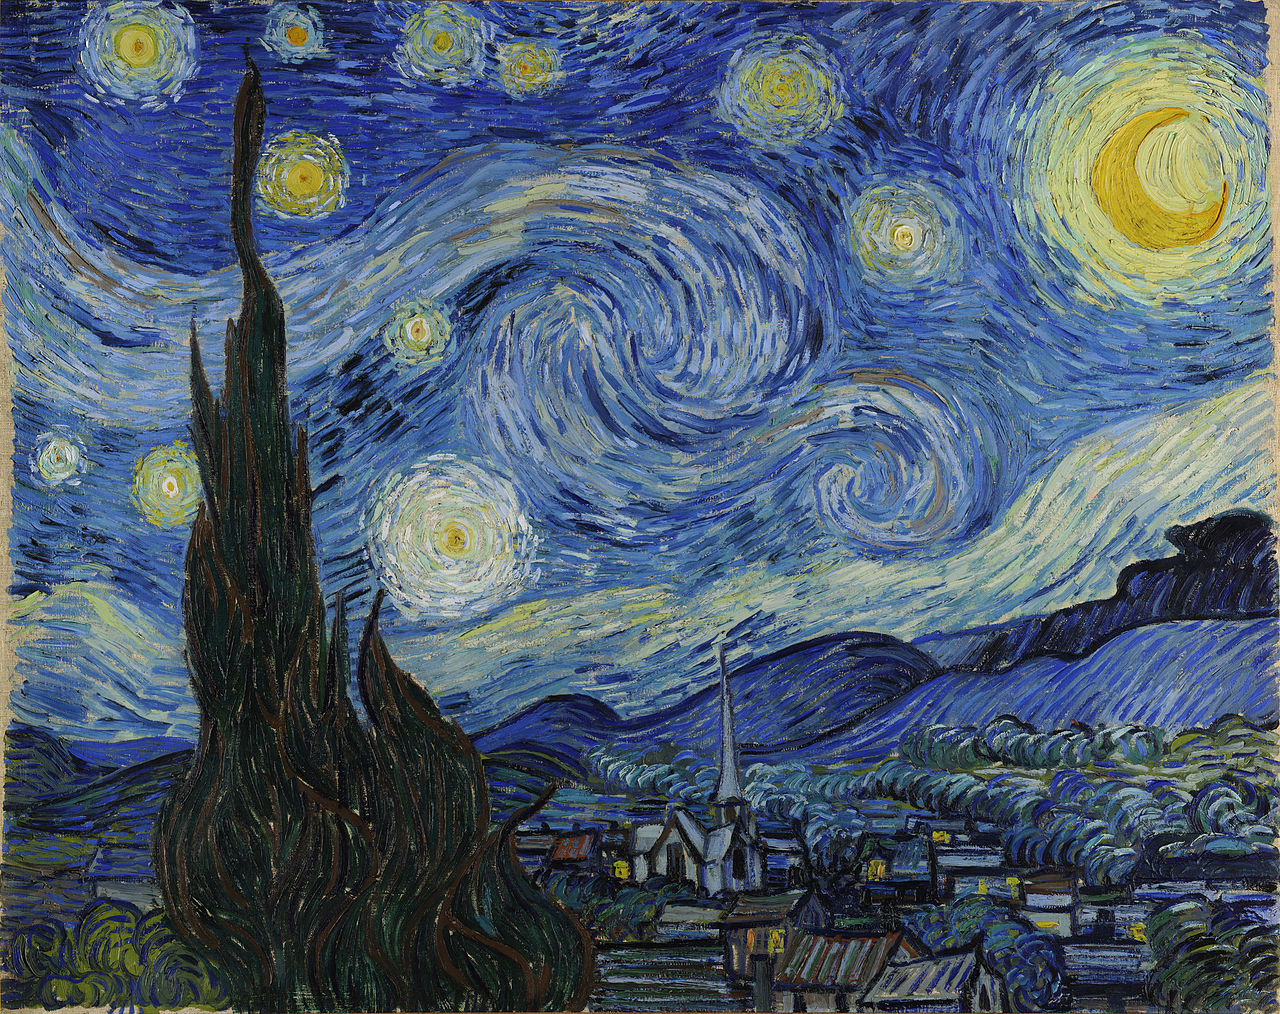
\includegraphics[height=5cm, width=\textwidth]{style1}
        \label{fig:content}
	\end{subfigure}
    \hfill
    \begin{subfigure}[b]{0.4\textwidth}
    	B
		\centering
        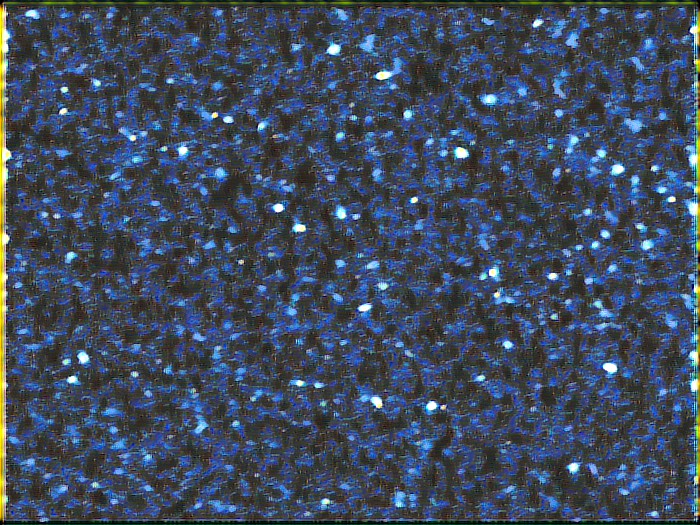
\includegraphics[height=5cm, width=\textwidth]{style_relu1_1}
        \label{fig:style_relu1_1}
	\end{subfigure}
    \begin{subfigure}[b]{0.4\textwidth}
    	C
		\centering
        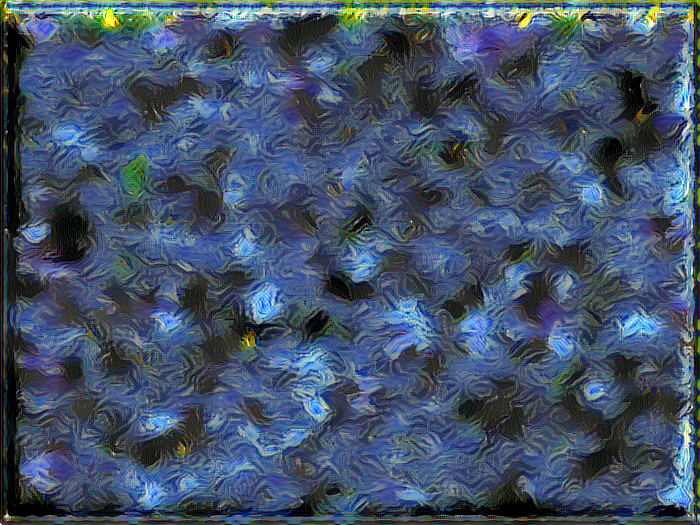
\includegraphics[height=5cm, width=\textwidth]{style_relu2_1}
        \label{fig:style_relu2_1}
	\end{subfigure}
    \hfill
    \begin{subfigure}[b]{0.4\textwidth}
    	D
		\centering
        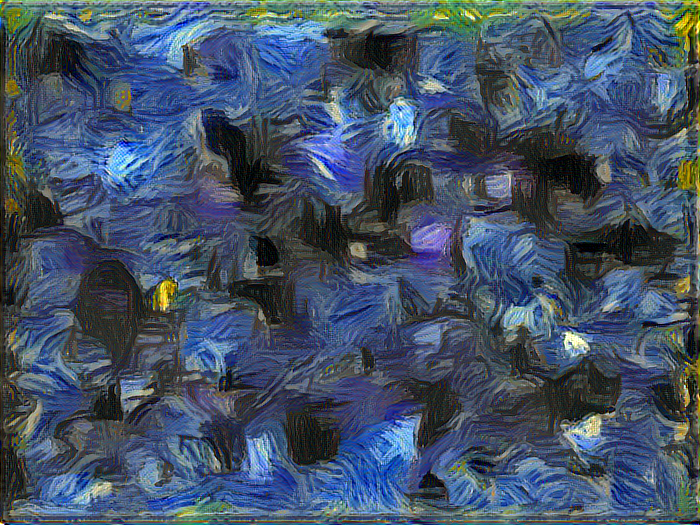
\includegraphics[height=5cm, width=\textwidth]{style_relu3_1}
        \label{fig:style_relu3_1}
	\end{subfigure}
    \begin{subfigure}[b]{0.4\textwidth}
    	E
		\centering
        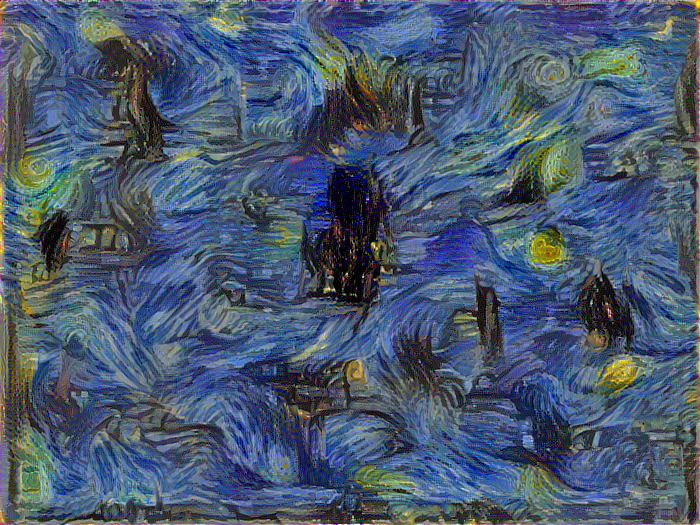
\includegraphics[height=5cm, width=\textwidth]{style_relu4_1}
        \label{fig:style_relu4_1}
	\end{subfigure}
    \hfill
    \begin{subfigure}[b]{0.4\textwidth}
    	F
		\centering
        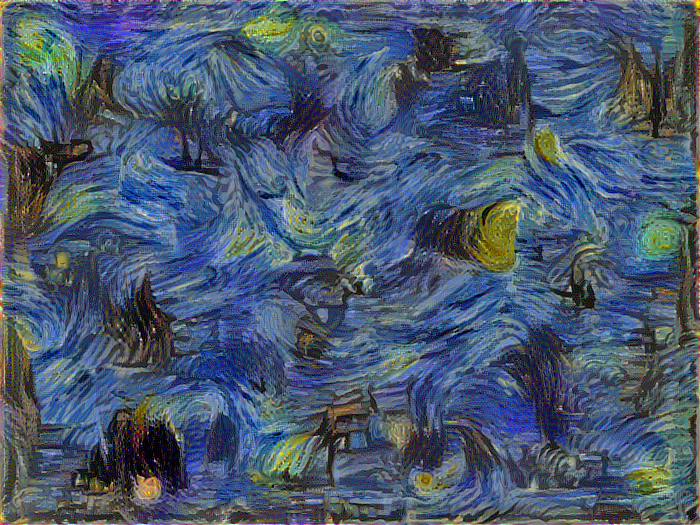
\includegraphics[height=5cm, width=\textwidth]{style_relu5_1}
        \label{fig:content_relu5_1}
	\end{subfigure}
    \caption{Generarea stilului. Figura $A$ este poza pentru care vreau să generez stilul, iar celelalte sunt pozele generate plecând de la o poză inițializată cu zgomot aleator. Pentru poza $B$ am folosit activările din layerul \textit{conv1{\_}1}, pentru poza $C$ am folosit layerele \textit{conv1{\_}1} și \textit{conv2{\_}1}, pentru poza $D$ am folosit layerele \textit{conv1{\_}1}, \textit{conv2{\_}1} și \textit{conv3{\_}1}, pentru poza $E$ am folosit layerele \textit{conv1{\_}1}, \textit{conv2{\_}1}, \textit{conv3{\_}1} și \textit{conv4{\_}1}, iar pentru poza $F$ am folosit layerele \textit{conv1{\_}1}, \textit{conv2{\_}1}, \textit{conv3{\_}1}, \textit{conv4{\_}1} și \textit{conv5{\_}1}. Peste activările acestor layere am aplicat ReLU. Se poate observa că pe măsură ce folosim layere aflate mai departe în rețea, obținem o textură a pozei inițiale, părți din obiectele acesteia apărând în textura generată.}
    \label{fig:style_rec}
\end{figure}

\section{Metodă}
În această secțiune voi defini o funcție de cost, propusă de Leon A. Gatys în articolul sau, A Neural Algorithm of Artistic Style \cite{gatys2015}, care ne va ajuta în generarea unei imagini care combină conținutul unei poze cu stilul alteia.

Această metodă presupune ca având ca date de intrare două poze, o poză în care se află conținutul pe care ni-l dorim în poza finala și o poză care conține stilul dorit să obținem o nouă poză artistică ce combină conținutul cu stilul pozelor de intrare.

Fie $\vec{x}$ o imagine inițializată cu zgomot aleator, $\vec{c}$ imaginea care conține conținutul pe care ni-l dorim și $\vec{s}$ imaginea care conține stilul, atunci $H^l$ este lungimea pozei la layerul $l$, $W^l$ este lățimea pozei la layerul $l$ și $C^l$ este numărul de canale/filtre ale pozei la layerul $l$. $F_{ijk}^l$ este activarea neuronului de la poziția $ijk$ din layerul $l$. Pentru pozele $\vec{x}$ și $\vec{c}$ considerăm matricele activărilor $X_{ijk}^l$, respectiv $C_{ijk}^l$. Atunci, funcția de cost pentru conținut, de care am vorbit în [\ref{ss:genc}] este definită astfel:

\begin{equation}
\label{eq:content_loss}
\mathcal{L}_{continut}(\vec{c}, \vec{x}) = \frac{1}{2H^{l}W^{l}C^{l}} \sum_{i, j, k}{(C_{ijk}^l - X_{ijk}^l)^2}
\end{equation}

La notațiile pentru ecuația [\ref{eq:content_loss}] mai adăugam câteva notații. Fie $N^l$ numărul de filtre pentru o poza din layerul $l$ și $M^l = H^{l} * W^{l}$. Atunci, matricea $FV^l \in \mathcal{R}^{N^{l} \times M^{l}}$ conține pe fiecare linie vectorul filtrului respectiv din layerul $l$, unde $FV_{ij}^l$ este activarea neuronului din filtrul $i$ la poziția $j$ în layerul $l$.

Pentru a putea construi funcția pentru stil, vom folosi matricele gram calculate pentru poza cu zgomot $\vec{x}$, respectiv poza care conține stilul $\vec{s}$. O matrice gram este definită astfel, fie $\vec{v_1}, \vec{v_2} ... \vec{v_n}$ vectori, atunci matricea gram este egală cu produsul scalar dintre fiecare doi vectori $Gram_{ij} = \langle {\vec{v_i}, \vec{v_j}} \rangle$ \cite{wiki_gram}

Pentru pozele $\vec{x}$ și $\vec{s}$ considerăm matricile $XV^l \in \mathcal{R}^{N^{l} \times M^{l}}$, respectiv $SV^l \in \mathcal{R}^{N^{l} \times M^{l}}$ și matricile gram $XG_{ij}^l = \displaystyle \sum_{k}{XV_{ik}^l XV_{jk}^l}$, respectiv $SG_{ij}^l = \displaystyle \sum_{k}{SV_{ik}^l SV_{jk}^l}$.

Pentru o mai bună înțelegere a matricelor gram, se pot vedea pozele [\ref{fig:unrolled_filters}, \ref{fig:gram_matrix}], luate din cursul lui Andrew Ng \cite{coursera_gram}.

\begin{figure}[H]
		\centering
        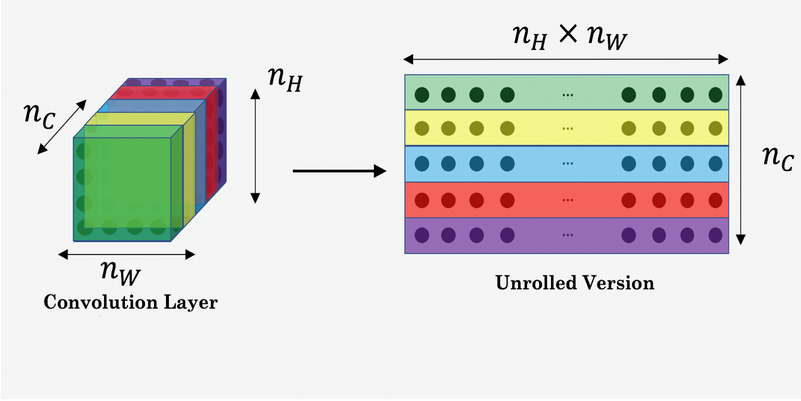
\includegraphics[width=\textwidth]{unrolled_filters}
        \caption{Filtrele salvate ca vectori. $N_H = H^l, N_W = W^l, N_C = C^l$. Aici se poate vedea o exemplificare a matricei $FV^l \in \mathcal{R}^{N^{l} \times M^{l}}$}
        \label{fig:unrolled_filters}
\end{figure}
\begin{figure}[H]
		\centering
        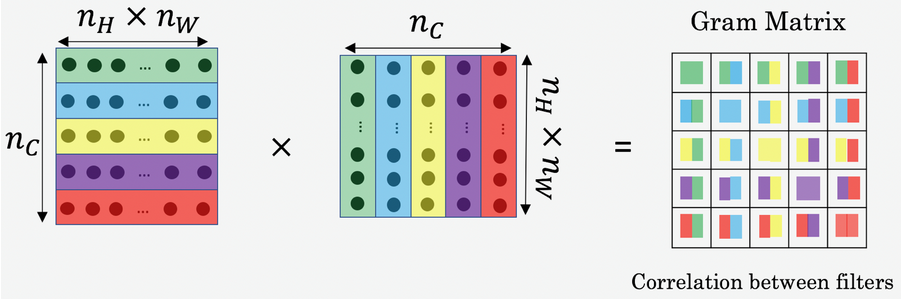
\includegraphics[width=\textwidth]{gram_matrix}
        \caption{Matricea Gram. $N_H = H^l, N_W = W^l, N_C = C^l$. Aici se poate vedea o exemplificare a matricei gram $Gram_{ij} = \langle {\vec{v_i}, \vec{v_j}} \rangle$}
        \label{fig:gram_matrix}
\end{figure}

Așadar, matricea gram calculează cât de mult apar 2 filtre împreuna într-o poza, fiind produsul dintre activările a doi neuroni care văd aceeași porțiune din imagine. Cu cât valoarea din matricea gram este mai mare, cu atât înseamnă că cele două filtre sunt mai corelate.

Având matricele gram calculate, costul dintr-un anumit layer poate fi construit astfel:
\begin{equation}
\label{eq:layer_style_loss}
E_l = \frac{1}{4(H^{l})^{2}(W^{l})^{2}(C^{l})^{2}} \sum_{i, j}{(SG_{ij}^l - XG_{ij}^l)^2}
\end{equation}

Atunci, funcția de cost pentru stil, de care am vorbit în [\ref{ss:gens}] este definită astfel:
\begin{equation}
\label{eq:style_loss}
\mathcal{L}_{stil}(\vec{s}, \vec{x}) = \sum_{l=1}^{L} w_l E_l
\end{equation}
unde $L$ este numărul de layere luate în considerare pentru generarea stilului, iar $w_l$ este un parametru care controlează importanța layerului $l$.

Pentru ca pozele generate să fie cât mai calitative, să nu prezinte zgomot, o să mai definesc o funcție de cost care calculează cât de mult zgomot este în imagine \cite{tvd}. Aceasta are următoarea formulă:

\begin{equation}
\label{eq:tv_loss}
\mathcal{L}_{zgomot}(\vec{x}) = \sum_{i, j} |x_{i+1, j} - x_{i, j}| + |x_{i, j + 1} - x{i, j}|
\end{equation}

Având definite costurile pentru zgomot, conținut și stil, costul total se definește astfel:
\begin{equation}
\label{eq:total_loss}
\mathcal{L}_{total}(\vec{c}, \vec{s}, \vec{x}) = \alpha \mathcal{L}_{continut}(\vec{c}, \vec{x}) + \beta \mathcal{L}_{stil}(\vec{s}, \vec{x}) + \gamma \mathcal{L}_{zgomot}(\vec{x})
\end{equation}
unde parametrii $\alpha$, $\beta$ și $\gamma$ controlează compromisul dintre conținut, stil și respectiv zgomot.

Pe baza funcției totale de cost vom optimiza pixelii unei poze inițializate cu zgomot aleator cu ajutorul algoritmului gradientului de coborâre astfel încât costul total să fie cât mai mic.

\section{Detalii de implementare}
Pentru a implementa metoda descrisă mai sus am folosit Python [\ref{sb:python}] și TensorFlow [\ref{sb:tensorflow}].
După cum am observat, rețelele convoluționale învață anumite reprezentări ale obiectelor dintr-o poză atunci cănd sunt antrenate pentru diferite sarcini. Astfel, pentru a putea calcula costurile definite în subcapitolul precedent ne vom folosi de activările din layerele unei rețele convoluționale care a fost antrenată să recunoască obiectele dintr-o poză. Antrenarea a avut loc pe baza a aproximativ 1,2 milioane de poze, obiectele din poze fiind clasificate în 1000 de categorii. În figura [\ref{fig:imagenet}] se pot observa câteva poze din setul de antrenare. Această rețea a fost folosită la competiția ImageNet din 2014 [\ref{sb:imagenet}], unde a obținut locul 2 la problema de clasificare, obținând o eroare egală cu $0.07$ și se numește VGG19 [\ref{fig:vgg19}], iar parametrii pe care i-a învățat rețeaua în timpul antrenării sunt făcuți publici de către autorii acesteia pe site-ul lor. \cite{parametri_vgg19} Din această rețea am folosit doar layerele convoluționale, fără cele conectate complet, iar în loc de \textit{maxpool} am folosit \textit{avgpool}, precum Leon A. Gatys, deoarece acesta a observat că această modificare produce rezultate mai satisfăcătoare.

\begin{figure}[H]
		\centering
        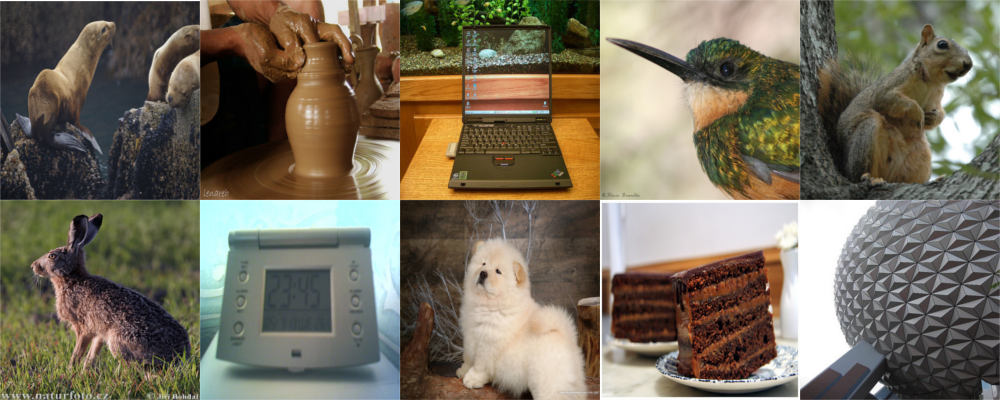
\includegraphics[height=5cm,width=\textwidth]{imagenet}
        \caption{Imagini din setul de antrenare ImageNet}
        \label{fig:imagenet}
\end{figure}

\begin{figure}[H]
		\centering
        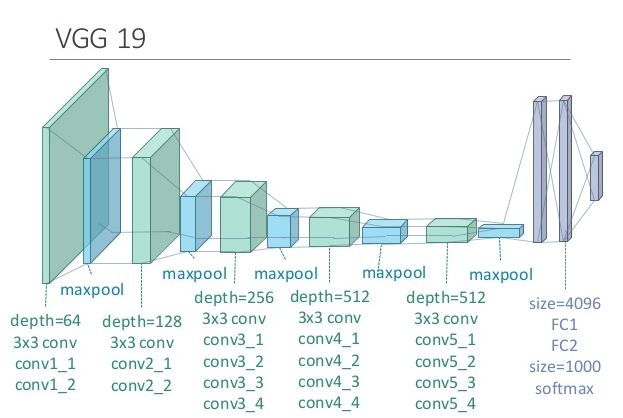
\includegraphics[height=6cm,width=\textwidth]{vgg19}
        \caption{Arhitectura rețelei neurale convoluționale VGG19 \cite{arh_vgg19}}
        \label{fig:vgg19}
\end{figure}

Algoritmul primește ca date de intrare două poze în spațiul de culori RGB, una cu conținutul dorit și alta cu stilul dorit. Având rețeaua de mai sus și cele două poze, am inițializat o poză de aceeași dimensiune cu cea a pozei de conținut folosind inițializarea Xavier [\ref{sb:xavier}], astfel, poza inițială prezintă zgomot aleator, pixelii acesteia având o distribuție uniformă, cu valori între $[-limita, limita]$, unde $limita = \sqrt{\frac{6}{H * W * C}}$, iar $H$ este lungimea pozei, $W$ este lățimea pozei și $C$ este numărul de canale ale pozei.

Apoi am normalizat cele trei poze pentru a avea aceeași distribuție ca cea pe care a fost antrenată rețeaua, și anume, pentru fiecare canal al pozei am scăzut valorile $[123.68, 116.779, 103.939]$, valori care reprezintă media canalelor RGB pentru pozele folosite la antrenare de rețeaua VGG19 și le-am trecut pe rând prin rețea și pentru fiecare am salvat ieșirile din layerul \textit{conv4{\_}2} pentru conținut și ieșirile din layerele \textit{conv1{\_}1}, \textit{conv2{\_}1}, \textit{conv3{\_}1}, \textit{conv4{\_}1}, \textit{conv5{\_}1} pentru stil. Acestea sunt numele layerelor din rețeaua VGG19. Peste aceste valori pe care le-am salvat am aplicat ReLU [\ref{sb:relu}] și am calculat costul cu ajutorul funcțiilor de cost definite, iar cu algoritmul gradientului de coborâre [\ref{sb:gradient_descent}] și a metodei backpropagation [sb:backpropagation] de calculare a gradienților am optimizat pixelii pozei inițiale astfel încât costul total să fie cât mai mic.

În imaginea [\ref{fig:vgg_workflow}] se poate observa procesul pe care l-am descris mai sus.

\begin{figure}[H]
		\centering
        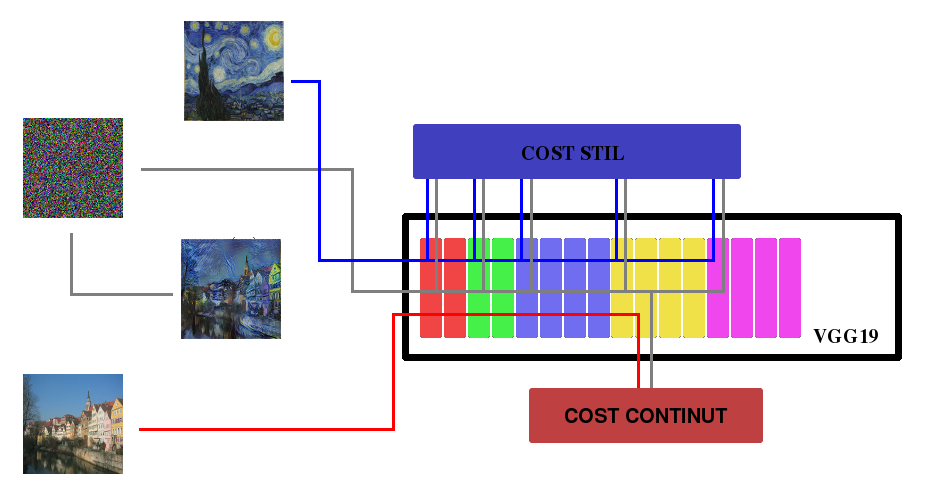
\includegraphics[width=\textwidth]{vgg_workflow}
        \caption{Workflow-ul algoritmului}
        \label{fig:vgg_workflow}
\end{figure}

Pentru toate rezultatele din acest capitol am repetat procedeul de mai sus timp de 2000 de iterații cu rata de învățare [\ref{sb:learning_rate}] egală cu 2 pentru a ajunge la rezultate satisfăcătoare. De asemenea, am ales $\alpha = 100$, $\beta = 1$, $\gamma = 0.03$ și $w_l = 0.2$ pentru toate layerele. Acești parametri i-am ales după mai multe încercări, în care am analizat pozele generate, după percepția mea, deoarece pentru acest timp de problemă nu există o metrică pentru a spune cât de bune sunt pozele generate. Pozele au fost redimensionate, păstrând raportul dintre lungime și lățime, la $max(lungime, latime) = 700$ de pixeli.

\subsection{Python}
\label{sb:python}
Python \cite{wiki_python} este un limbaj de programare, creat de Guido van Rossum în anul 1991. Este suportat de mai multe sisteme de operare fiind un limbaj de programare ușor  de folosit și care oferă posibilitatea de a scrie programe complexe, într-o maniera elegantă. Python este folosit de majoritatea celor care doresc să creeze programe ce folosesc învățarea automată.

\subsection{TensorFlow}
\label{sb:tensorflow}
TensorFlow \cite{wiki_tf} a fost creat de către cercetătorii din echipa Google Brain. Această librărie, prin funcțiile pe care le deține, ca de exemplu calcularea gradienților sau crearea de layere într-o rețea, oferă posibilitatea de a construi ușor programe ce folosesc învățarea automată. Tensorflow este folosit activ de cei de la Google și de asemenea este și open-source, fapt ce constituie un plus, deoarece datorită numărului mare de contribuitori este îmbunătățit continuu.

\subsection{ImageNet}
\label{sb:imagenet}
ImageNet \cite{imagenet} este o bază de date ce conține milioane de poze adnotate de către oameni, imagini destinate pentru diferite probleme legate de învățarea automată. Începând cu anul 2010, în fiecare an se organizează un concurs numit ImageNet Large Scale Visual Recognition Challenge (ILSVRC) în care diferiți cercetători încearcă să obțină rezultate cât mai bune la probleme de genul: clasificarea obiectelor dintr-o poză sau localizarea obiectelor.

\subsection{Inițializarea Xavier}
\label{sb:xavier}
\cite{coursera_deep_learning} O problemă cu care se confruntă rețelele convoluționale foarte adânci este modul în care sunt inițializate filtrele. Dacă acestea sunt inițializate cu valori prea mici, atunci de-a lungul rețelei, este posibil să devină foarte aproape de zero, astfel rețeaua nemaiputând învăța. Pe de altă parte, dacă sunt prea mari, atunci acestea tind să devină prea mari de-a lungul rețelei ca să mai fie folositoare. În articolul său \cite{glorot2010}, Xavier Glorot propune o formulă de inițializare a filtrelor care s-a dovedit a fi fiabilă în practică. Această inițializare are rolul de a ține valorile dintr-un anumit filtru într-un anumit interval, valorile având o distribuție uniformă sau normală. Formula pentru variație în cazul când dorim ca valorile să aibă o distribuție uniformă este:

\begin{equation}
\label{eq:xavier}
variatie = \sqrt{\frac{6}{intrari + iesiri}}
\end{equation}

Unde $intrari$ reprezintă câte valori intră în layerul respectiv, iar $iesiri$ câte valori ies din layerul respectiv.

\subsection{ReLU}
\label{sb:relu}
Rectified linear unit (ReLU) \cite{wiki_relu} este o funcție de activare neliniară. Aceasta se aplică pe valorile de ieșire ale layerelor. Este inspirată din biologie și din cum se crede că funcționează transmiterea de informație în creier. Atunci când un neuron are o valoare negativă, după aplicarea funcției ReLU acesta are valoarea 0, însemnând ca este inactiv, iar când valoarea unui neuron este pozitivă, activarea acestuia este fix valoarea lui.

\begin{equation}
\label{eq:relu}
f(x) = max(0, x)
\end{equation}

\subsection{Coborâre pe gradient}
\label{sb:gradient_descent}
Coborârea pe gradient \cite{coursera_deep_learning} este un algoritm de minimizare a unei funcții care depinde de mai multe variabile. Să presupunem că funcția de cost este următoarea $\mathcal{L}(x_1, x_2 ... x_n)$. Atunci, pentru a minimiza această funcție vom aplica următorul algoritm pentru modificarea variabilelor de care depinde.

\begin{equation}
\label{eq:gradient_descent}
x_i = x_i - \alpha * \frac{\partial}{\partial{x_i}}\mathcal{L}
\end{equation}

Unde $\frac{\partial}{\partial{x_i}}\mathcal{L}$ este derivata parțială a funcției $\mathcal{L}$ în raport cu variabila $x_i$. Derivata reprezintă panta tangentei la graficul funcției, și indică direcția funcției, dacă aceasta crește sau descrește. Iar $\alpha$ este rata de învățare.

\subsection{Backpropagation}
\label{sb:backpropagation}
\cite{coursera_deep_learning} Așa cum am văzut la algoritmul coborârii pe gradient, pentru a minimiza o funcție de cost $\mathcal{L}(x_1, x_2 ... x_n)$, este nevoie să calculăm derivatele parțiale $\frac{\partial}{\partial{x_i}}\mathcal{L}$. Plecând de la rezultatul funcției de cost, cu ajutorul acestei metode se propagă înapoi în rețea eroarea până la variabilele de care depinde această funcție care sunt optimizate după formula [\ref{eq:gradient_descent}].

\subsection{Optimizatorul Adam}
\label{sb:adam_optimizer}
Optimizatorul Adam \cite{coursera_deep_learning} este o variantă îmbunătățită a algoritmului coborârii pe gradient făcând ca învățarea să meargă mai repede. O problemă a coborârii pe gradient este aceea că face mulți pași până a ajunge să conveargă către minim. Optimizatorul Adam se folosește de valorile anterioare ale gradienților, și intuitiv, vede un trend pe care îl urmează gradienții, putând la un anumit moment să facă un pas mai mare decât ar face algoritmul coborârii pe gradient. Formula acestuia la pasul $t$ este următoarea:

\begin{equation}
V_t = \beta1 * V_{t-1} + (1 - \beta1) * \frac{\partial}{\partial{x_i}}\mathcal{L}
\end{equation}
\begin{equation}
S_t = \beta2 * S_{t-1} + (1 - \beta2) * \frac{\partial}{\partial{x_i}}\mathcal{L} * \frac{\partial}{\partial{x_i}}\mathcal{L}
\end{equation}
\begin{equation}
\label{eq:adam}
x_i = x_i - \alpha * \frac{V_t}{\sqrt{S_t} + \epsilon}
\end{equation}

Unde, de obicei, $\beta1 = 0.9$, asta însemnând aproximativ că $V_t$ calculează media ultimilor 10 gradienți, $\beta2 = 0.999$, $\epsilon = 1e-08$, acesta este folosit în cazul în care $S_t = 0$ și să se evite împărțirea la 0, iar $\alpha$ este rata de învățare.

\subsection{Rata de învățare}
\label{sb:learning_rate}
Rata de învățare \cite{coursera_deep_learning} este folosită în formula algoritmilor de optimizare. Aceasta controlează cat de mult să fie modificată o variabilă pentru a optimiza funcția țintă. O valoare mica a acestei rate, înseamnă că variabila respectivă se va modifica foarte puțin, fiind necesar un timp mai mare pentru ca funcția să conveargă către minim. Pe de altă parte, dacă rata de învățarea este foarte mare, atunci este posibil ca funcția să nu mai ajungă să conveargă, deoarece variabila este modificată foarte mult.

\newpage
\section{Rezultate și comparații}
\begin{figure}[H]
	\centering
    \begin{subfigure}[b]{0.75\textwidth}
		\centering
        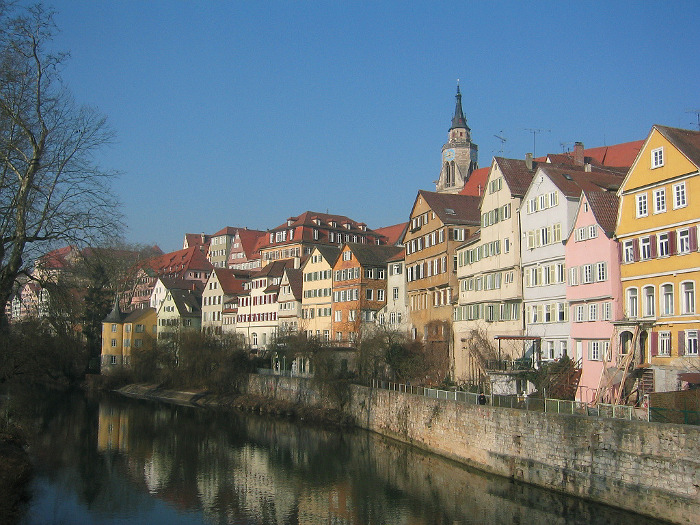
\includegraphics[height=4.5cm, width=0.7\textwidth]{content1}
        \label{fig:content}
        \caption{Neckarfront, Tübingen, Germania, autor Andreas Praefcke.}
	\end{subfigure}
    \begin{subfigure}[b]{0.5\textwidth}
		\centering
        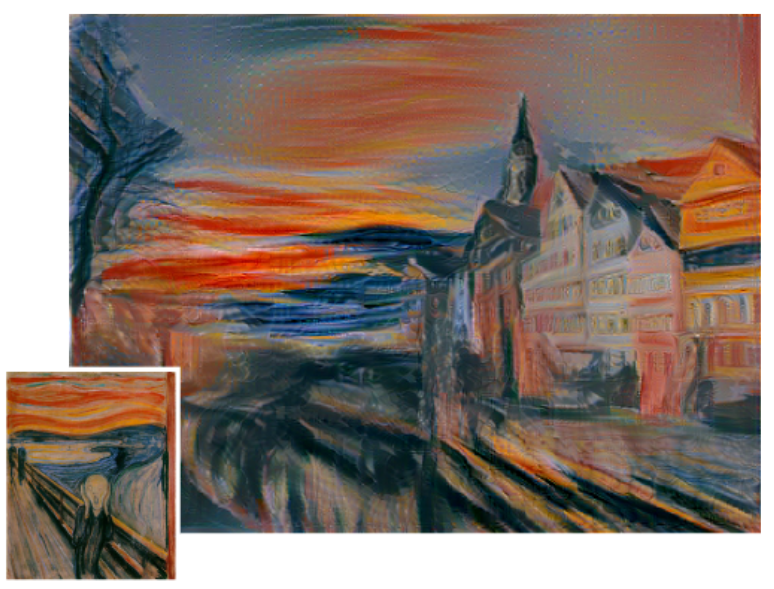
\includegraphics[height=4.5cm, width=1.1\textwidth]{anaoas_c1s2_gatys}
        \label{fig:anaoas_c1s2_gatys}
        \caption{The Scream, Edvard Munch, 1893.}
	\end{subfigure}
    \hfill
    \begin{subfigure}[b]{0.4\textwidth}
		\centering
        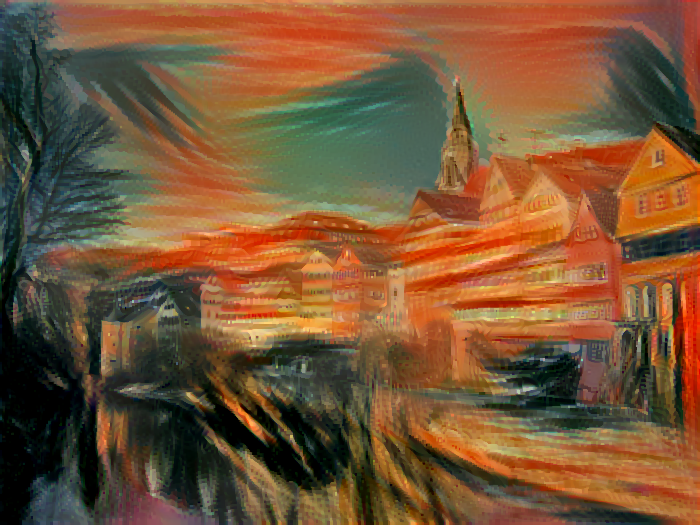
\includegraphics[height=4.5cm, width=1.2\textwidth]{anaoas_c1s2}
        \label{fig:anaoas_c1s2}
	\end{subfigure}
    \begin{subfigure}[b]{0.5\textwidth}
		\centering
        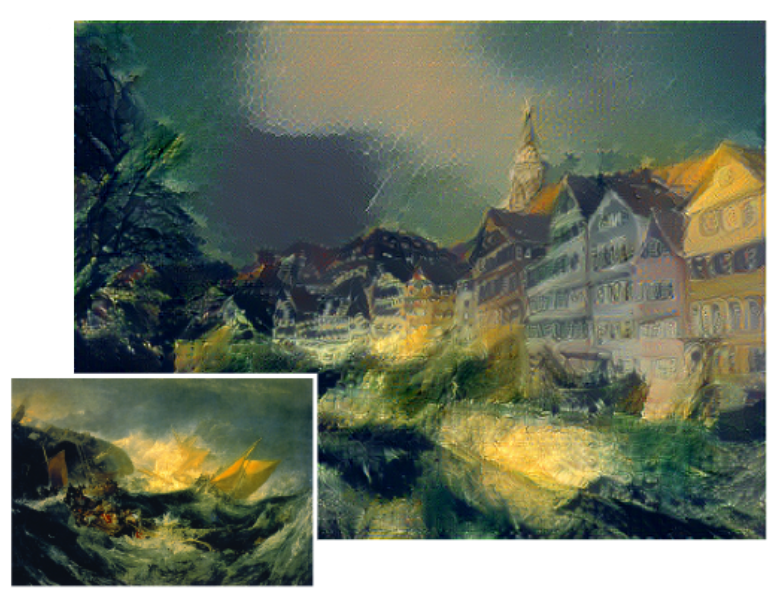
\includegraphics[height=4.5cm, width=1.1\textwidth]{anaoas_c1s3_gatys}
        \label{fig:anaoas_c1s3_gatys}
        \caption{The Shipwreck of the Minotaur, J.M.W. Turner, 1805}
	\end{subfigure}
    \hfill
    \begin{subfigure}[b]{0.4\textwidth}
		\centering
        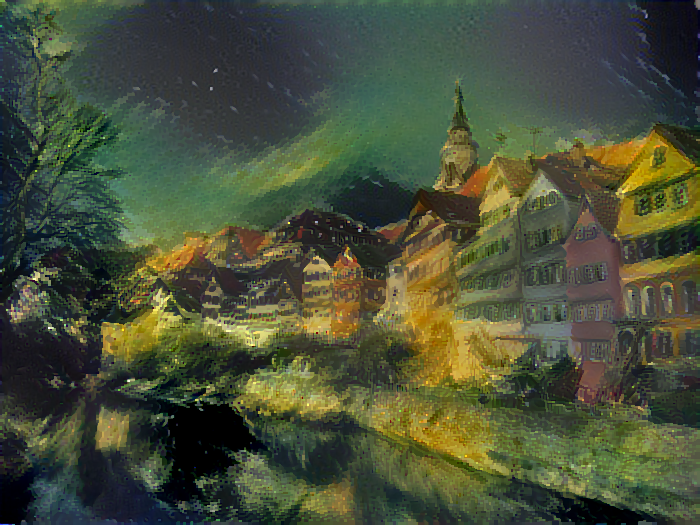
\includegraphics[height=5cm, width=1.2\textwidth]{anaoas_c1s3}
        \label{fig:anaoas_c1s3}
	\end{subfigure}
    \caption{Pe coloana din stânga sunt rezultatele luate din articolul lui Leon A. Gatys, iar pe coloana din dreapta sunt rezultatele obținute de mine. Pozele diferă deoarece contează dimensiunea imaginilor între care s-a realizat transferul de stil sau modul în care a fost implementat algoritmul. Fiindcă nu există un mod obiectiv pentru a decide care imagini sunt mai artistice, ambele variante sunt valabile.}
\end{figure}

\begin{figure}[H]
	\centering
    \begin{subfigure}[b]{0.5\textwidth}
		\centering
        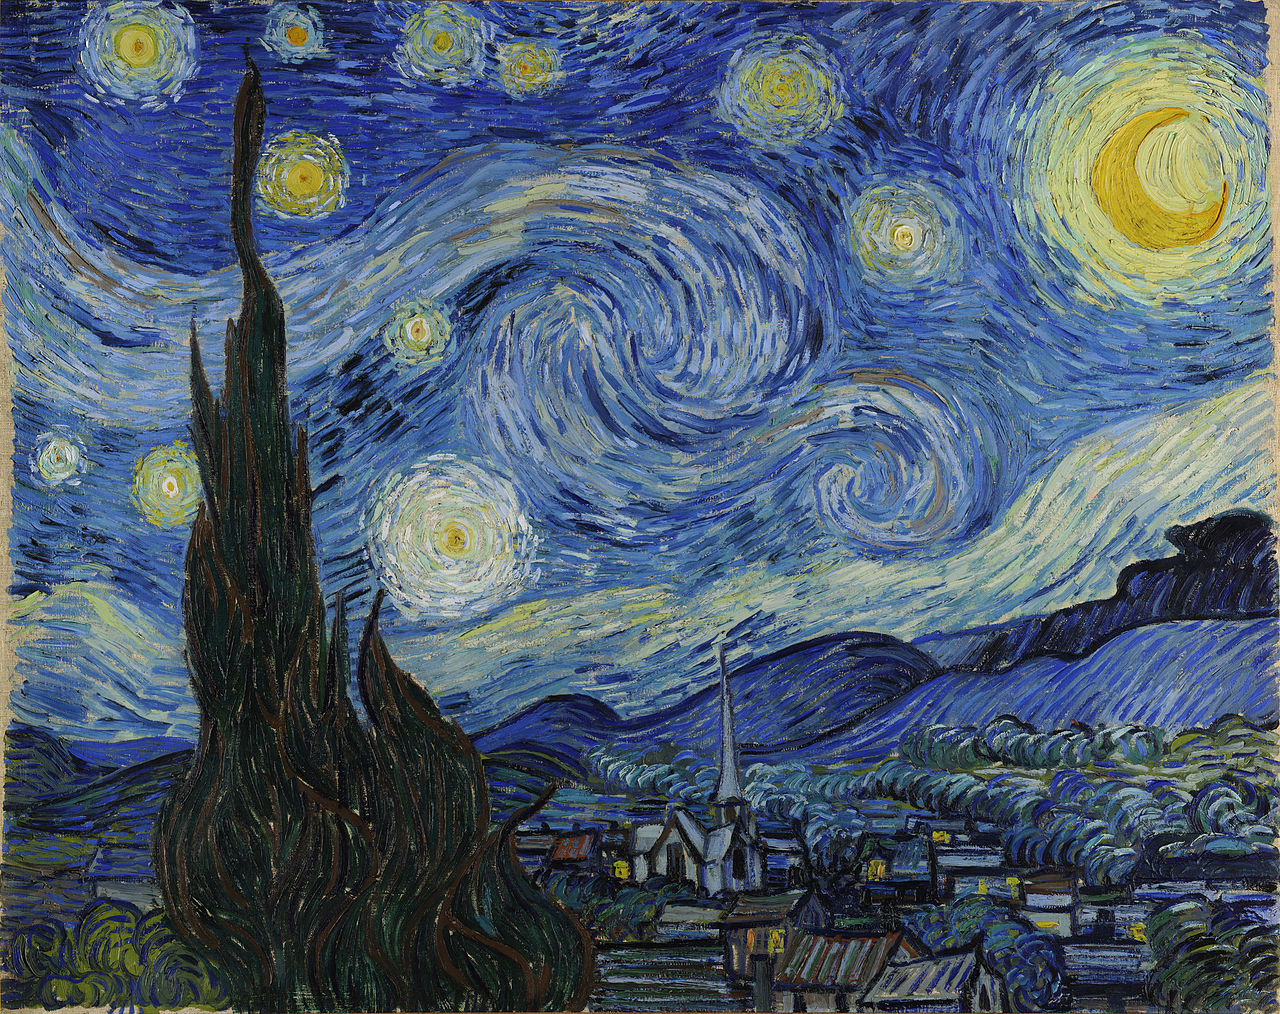
\includegraphics[height=2.5cm, width=0.7\textwidth]{style1}
        \label{fig:anaoas_style1}
        \caption{The Starry Night, Vincent van Gogh, 1889}
	\end{subfigure}
    \hfill
    \begin{subfigure}[b]{0.4\textwidth}
		\centering
        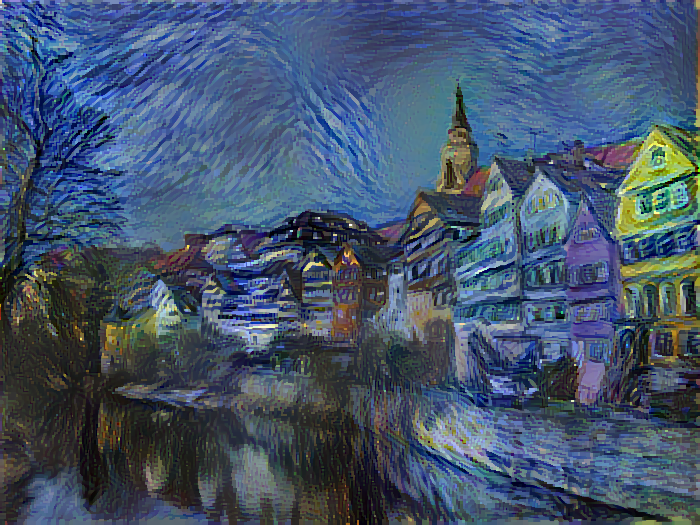
\includegraphics[height=4cm, width=1.1\textwidth]{anaoas_c1s1}
        \label{fig:anaoas_c1s1}
	\end{subfigure}
    \begin{subfigure}[b]{0.5\textwidth}
		\centering
        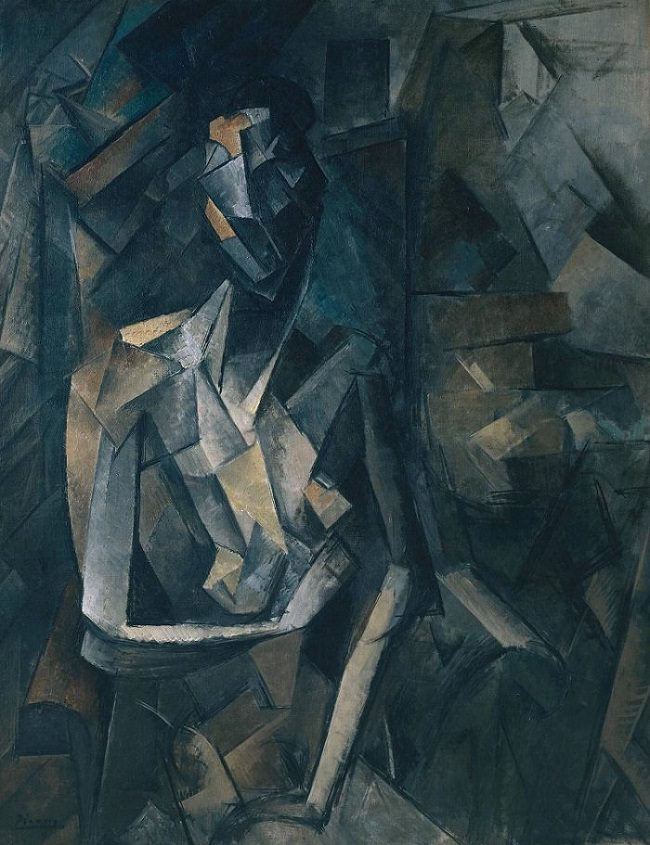
\includegraphics[height=2.5cm, width=0.7\textwidth]{style4}
        \label{fig:anaoas_style4}
        \caption{Femme nue assise, Pablo Picasso, 1910}
	\end{subfigure}
    \hfill
    \begin{subfigure}[b]{0.4\textwidth}
		\centering
        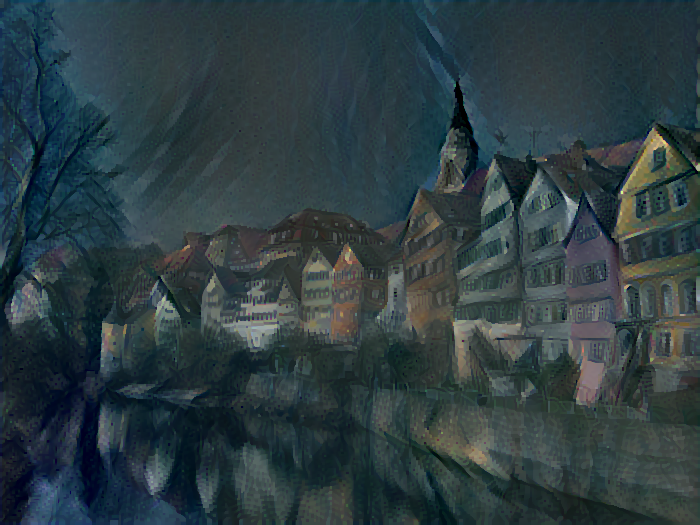
\includegraphics[height=4cm, width=1.1\textwidth]{anaoas_c1s4}
        \label{fig:anaoas_c1s4}
	\end{subfigure}
    \begin{subfigure}[b]{0.5\textwidth}
		\centering
        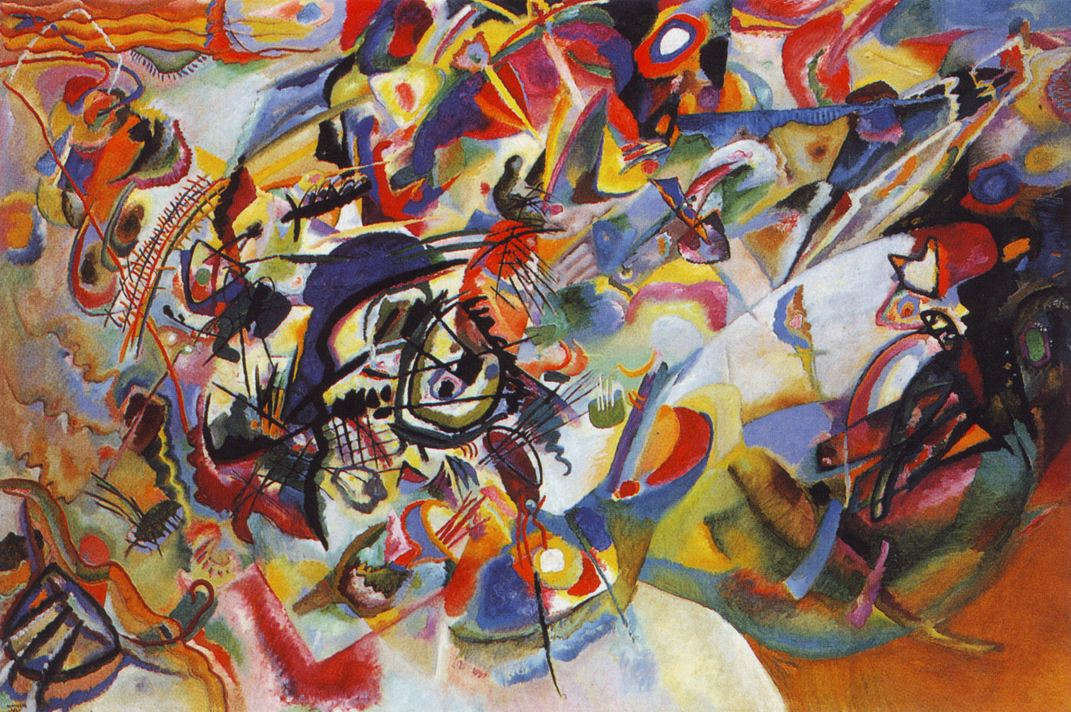
\includegraphics[height=2.5cm, width=0.7\textwidth]{style5}
        \label{fig:anaoas_style5}
        \caption{Composition VII, Wassily Kandinsky, 1913}
	\end{subfigure}
    \hfill
    \begin{subfigure}[b]{0.4\textwidth}
		\centering
        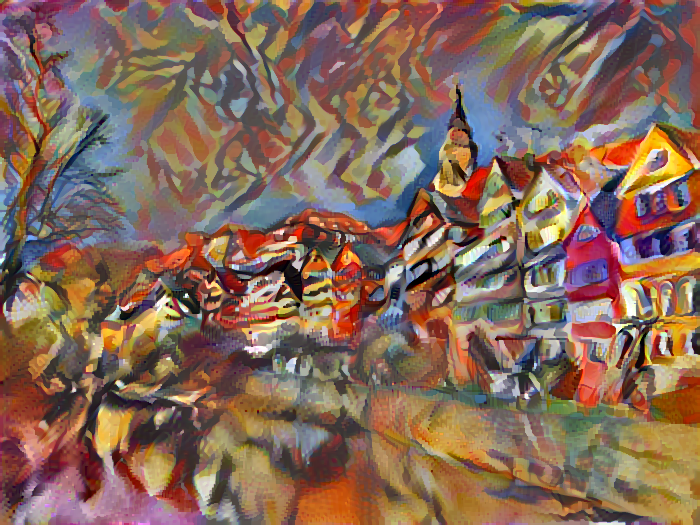
\includegraphics[height=4cm, width=1.1\textwidth]{anaoas_c1s5}
        \label{fig:anaoas_c1s5}
	\end{subfigure}
    \begin{subfigure}[b]{0.5\textwidth}
		\centering
        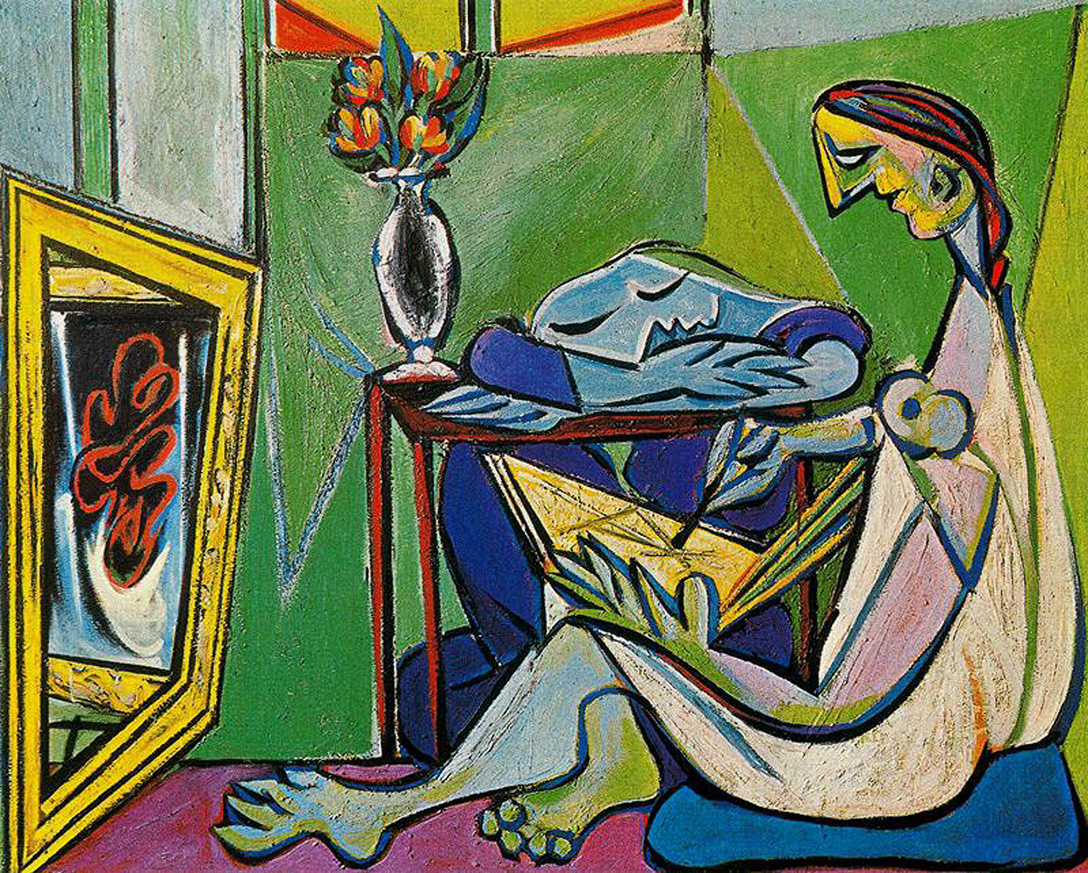
\includegraphics[height=2.5cm, width=0.7\textwidth]{style6}
        \label{fig:anaoas_style6}
        \caption{The Muse, Pablo Picasso, 1935}
	\end{subfigure}
    \hfill
    \begin{subfigure}[b]{0.4\textwidth}
		\centering
        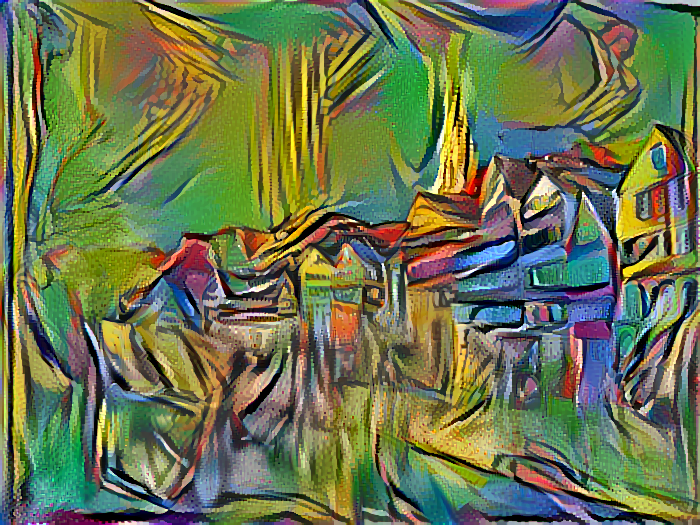
\includegraphics[height=4cm, width=1.1\textwidth]{anaoas_c1s6}
        \label{fig:anaoas_c1s6}
	\end{subfigure}
    \begin{subfigure}[b]{0.5\textwidth}
		\centering
        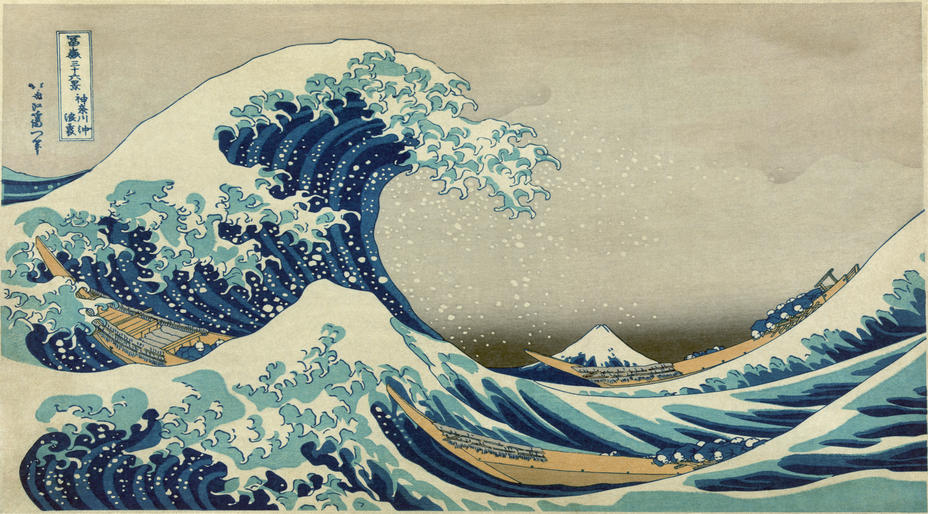
\includegraphics[height=2.5cm, width=0.7\textwidth]{style7}
        \label{fig:anaoas_style7}
        \caption{The Great Wave off Kanagawa, Hokusai, 1829-1832}
	\end{subfigure}
    \hfill
    \begin{subfigure}[b]{0.4\textwidth}
		\centering
        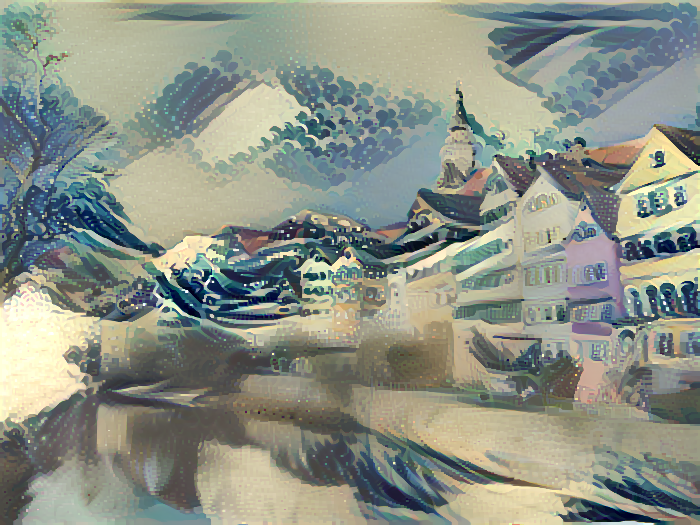
\includegraphics[height=4cm, width=1.1\textwidth]{anaoas_c1s7}
        \label{fig:anaoas_c1s7}
	\end{subfigure}
\end{figure}

\begin{figure}[H]
	\centering
    \begin{subfigure}[b]{0.19\textwidth}
		\centering
        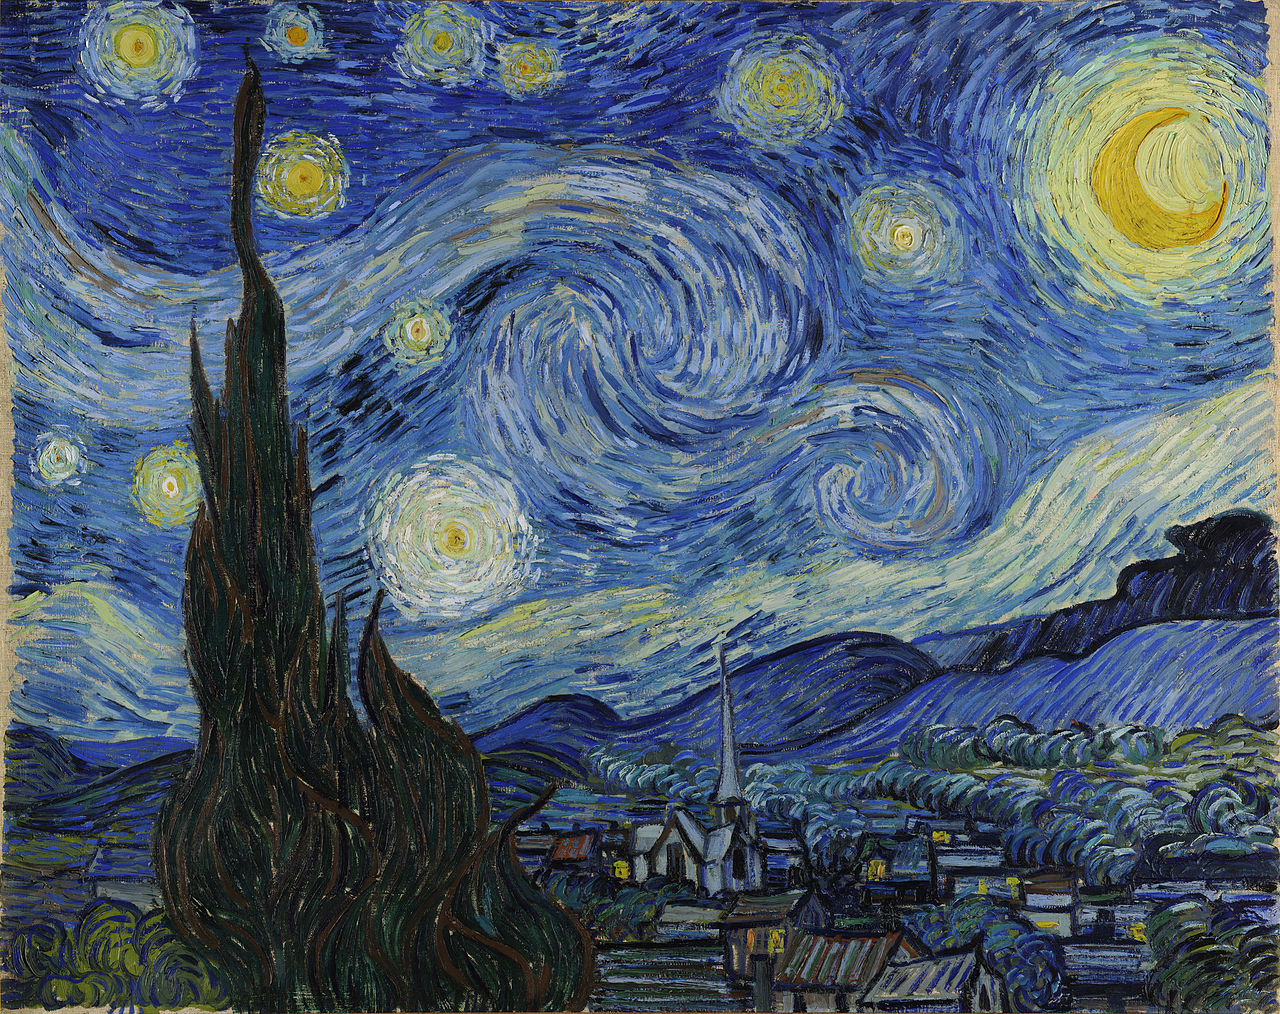
\includegraphics[height=2.5cm, width=1\textwidth]{style1}
        \label{fig:anaoas_style1}
	\end{subfigure}
    \hfill
    \begin{subfigure}[b]{0.19\textwidth}
		\centering
        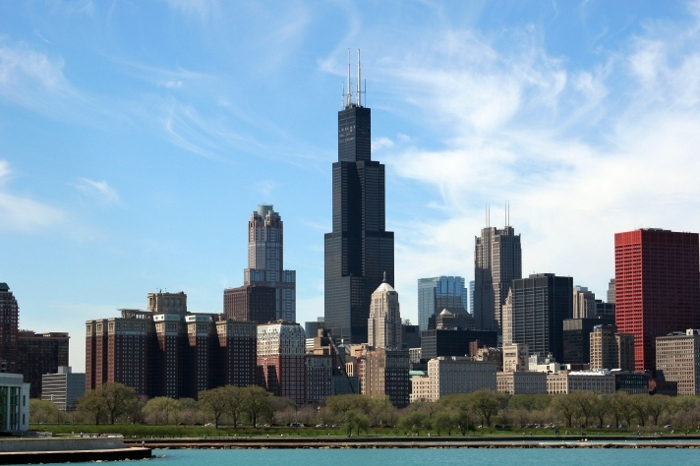
\includegraphics[height=2.5cm, width=1\textwidth]{content2}
        \label{fig:anaoas_conten2}
	\end{subfigure}
    \hfill
    \begin{subfigure}[b]{0.19\textwidth}
		\centering
        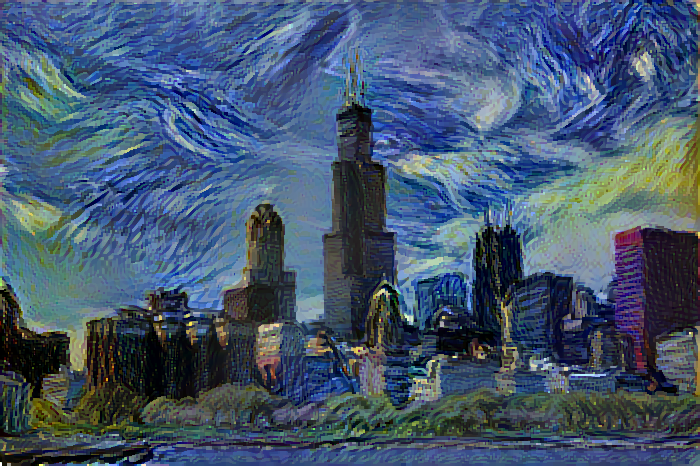
\includegraphics[height=2.5cm, width=1\textwidth]{anaoas_c2s1}
        \label{fig:anaoas_c2s1}
	\end{subfigure}
    \hfill
    \begin{subfigure}[b]{0.19\textwidth}
		\centering
        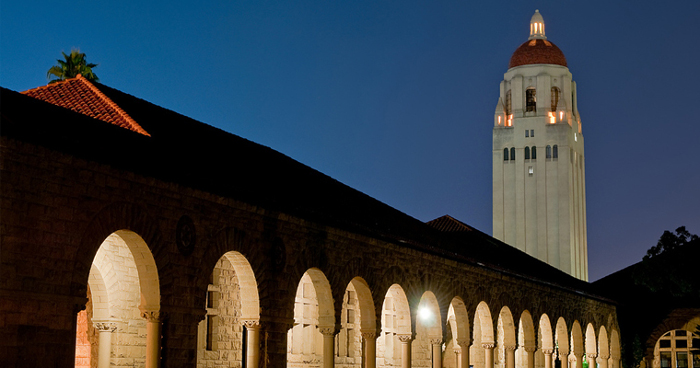
\includegraphics[height=2.5cm, width=1\textwidth]{content3}
        \label{fig:anaoas_conten3}
	\end{subfigure}
    \hfill
    \begin{subfigure}[b]{0.19\textwidth}
		\centering
        \includegraphics[height=2.5cm, width=1\textwidth]{anaoas_c3s1}
        \label{fig:anaoas_c3s1}
	\end{subfigure}
    \begin{subfigure}[b]{0.19\textwidth}
		\centering
        \includegraphics[height=2.5cm, width=1\textwidth]{style2}
        \label{fig:anaoas_style2}
	\end{subfigure}
    \hfill
    \begin{subfigure}[b]{0.19\textwidth}
		\centering
        \includegraphics[height=2.5cm, width=1\textwidth]{content2}
        \label{fig:anaoas_conten2}
	\end{subfigure}
    \hfill
    \begin{subfigure}[b]{0.19\textwidth}
		\centering
        \includegraphics[height=2.5cm, width=1\textwidth]{anaoas_c2s2}
        \label{fig:anaoas_c2s2}
	\end{subfigure}
    \hfill
    \begin{subfigure}[b]{0.19\textwidth}
		\centering
        \includegraphics[height=2.5cm, width=1\textwidth]{content3}
        \label{fig:anaoas_conten3}
	\end{subfigure}
    \hfill
    \begin{subfigure}[b]{0.19\textwidth}
		\centering
        \includegraphics[height=2.5cm, width=1\textwidth]{anaoas_c3s2}
        \label{fig:anaoas_c3s2}
	\end{subfigure}
    \begin{subfigure}[b]{0.19\textwidth}
		\centering
        \includegraphics[height=2.5cm, width=1\textwidth]{style3}
        \label{fig:anaoas_style3}
	\end{subfigure}
    \hfill
    \begin{subfigure}[b]{0.19\textwidth}
		\centering
        \includegraphics[height=2.5cm, width=1\textwidth]{content2}
        \label{fig:anaoas_conten2}
	\end{subfigure}
    \hfill
    \begin{subfigure}[b]{0.19\textwidth}
		\centering
        \includegraphics[height=2.5cm, width=1\textwidth]{anaoas_c2s3}
        \label{fig:anaoas_c2s3}
	\end{subfigure}
    \hfill
    \begin{subfigure}[b]{0.19\textwidth}
		\centering
        \includegraphics[height=2.5cm, width=1\textwidth]{content3}
        \label{fig:anaoas_conten3}
	\end{subfigure}
    \hfill
    \begin{subfigure}[b]{0.19\textwidth}
		\centering
        \includegraphics[height=2.5cm, width=1\textwidth]{anaoas_c3s3}
        \label{fig:anaoas_c3s3}
	\end{subfigure}
    \begin{subfigure}[b]{0.19\textwidth}
		\centering
        \includegraphics[height=2.5cm, width=1\textwidth]{style4}
        \label{fig:anaoas_style4}
	\end{subfigure}
    \hfill
    \begin{subfigure}[b]{0.19\textwidth}
		\centering
        \includegraphics[height=2.5cm, width=1\textwidth]{content2}
        \label{fig:anaoas_conten2}
	\end{subfigure}
    \hfill
    \begin{subfigure}[b]{0.19\textwidth}
		\centering
        \includegraphics[height=2.5cm, width=1\textwidth]{anaoas_c2s4}
        \label{fig:anaoas_c2s4}
	\end{subfigure}
    \hfill
    \begin{subfigure}[b]{0.19\textwidth}
		\centering
        \includegraphics[height=2.5cm, width=1\textwidth]{content3}
        \label{fig:anaoas_conten3}
	\end{subfigure}
    \hfill
    \begin{subfigure}[b]{0.19\textwidth}
		\centering
        \includegraphics[height=2.5cm, width=1\textwidth]{anaoas_c3s4}
        \label{fig:anaoas_c3s4}
	\end{subfigure}
    \begin{subfigure}[b]{0.19\textwidth}
		\centering
        \includegraphics[height=2.5cm, width=1\textwidth]{style5}
        \label{fig:anaoas_style5}
	\end{subfigure}
    \hfill
    \begin{subfigure}[b]{0.19\textwidth}
		\centering
        \includegraphics[height=2.5cm, width=1\textwidth]{content2}
        \label{fig:anaoas_conten2}
	\end{subfigure}
    \hfill
    \begin{subfigure}[b]{0.19\textwidth}
		\centering
        \includegraphics[height=2.5cm, width=1\textwidth]{anaoas_c2s5}
        \label{fig:anaoas_c2s5}
	\end{subfigure}
    \hfill
    \begin{subfigure}[b]{0.19\textwidth}
		\centering
        \includegraphics[height=2.5cm, width=1\textwidth]{content3}
        \label{fig:anaoas_conten3}
	\end{subfigure}
    \hfill
    \begin{subfigure}[b]{0.19\textwidth}
		\centering
        \includegraphics[height=2.5cm, width=1\textwidth]{anaoas_c3s5}
        \label{fig:anaoas_c3s5}
	\end{subfigure}
    \begin{subfigure}[b]{0.19\textwidth}
		\centering
        \includegraphics[height=2.5cm, width=1\textwidth]{style6}
        \label{fig:anaoas_style6}
	\end{subfigure}
    \hfill
    \begin{subfigure}[b]{0.19\textwidth}
		\centering
        \includegraphics[height=2.5cm, width=1\textwidth]{content2}
        \label{fig:anaoas_conten2}
	\end{subfigure}
    \hfill
    \begin{subfigure}[b]{0.19\textwidth}
		\centering
        \includegraphics[height=2.5cm, width=1\textwidth]{anaoas_c2s6}
        \label{fig:anaoas_c2s6}
	\end{subfigure}
    \hfill
    \begin{subfigure}[b]{0.19\textwidth}
		\centering
        \includegraphics[height=2.5cm, width=1\textwidth]{content3}
        \label{fig:anaoas_conten3}
	\end{subfigure}
    \hfill
    \begin{subfigure}[b]{0.19\textwidth}
		\centering
        \includegraphics[height=2.5cm, width=1\textwidth]{anaoas_c3s6}
        \label{fig:anaoas_c3s6}
	\end{subfigure}
    \begin{subfigure}[b]{0.19\textwidth}
		\centering
        \includegraphics[height=2.5cm, width=1\textwidth]{style7}
        \label{fig:anaoas_style7}
	\end{subfigure}
    \hfill
    \begin{subfigure}[b]{0.19\textwidth}
		\centering
        \includegraphics[height=2.5cm, width=1\textwidth]{content2}
        \label{fig:anaoas_conten2}
	\end{subfigure}
    \hfill
    \begin{subfigure}[b]{0.19\textwidth}
		\centering
        \includegraphics[height=2.5cm, width=1\textwidth]{anaoas_c2s7}
        \label{fig:anaoas_c2s7}
	\end{subfigure}
    \hfill
    \begin{subfigure}[b]{0.19\textwidth}
		\centering
        \includegraphics[height=2.5cm, width=1\textwidth]{content3}
        \label{fig:anaoas_conten3}
	\end{subfigure}
    \hfill
    \begin{subfigure}[b]{0.19\textwidth}
		\centering
        \includegraphics[height=2.5cm, width=1\textwidth]{anaoas_c3s7}
        \label{fig:anaoas_c3s7}
	\end{subfigure}
    \caption{}
    \label{fig:anaoas_diverse_rezultate}
\end{figure}

\begin{figure}[h]
	\centering
    \begin{subfigure}[b]{0.19\textwidth}
		\centering
        \includegraphics[height=2.8cm, width=1\textwidth]{style1}
        \label{fig:anaoas_style1}
        \caption{}
	\end{subfigure}
    \hfill
    \begin{subfigure}[b]{0.19\textwidth}
		\centering
        \includegraphics[height=2.8cm, width=1\textwidth]{content1}
        \label{fig:anaoas_conten1}
        \caption{}
	\end{subfigure}
    \hfill
    \begin{subfigure}[b]{0.19\textwidth}
		\centering
        \includegraphics[height=2.8cm, width=1\textwidth]{anaoas_c1s1}
        \label{fig:anaoas_c1s1}
        \caption{}
	\end{subfigure}
    \hfill
    \begin{subfigure}[b]{0.19\textwidth}
		\centering
        \includegraphics[height=2.8cm, width=1\textwidth]{anaoas_c1s1_stil400}
        \label{fig:anaoas_c1s1_stil400}
        \caption{}
	\end{subfigure}
    \hfill
    \begin{subfigure}[b]{0.19\textwidth}
		\centering
        \includegraphics[height=2.8cm, width=1\textwidth]{anaoas_c1s1_stil1400}
        \label{fig:anaoas_c1s1_stil1400}
        \caption{}
	\end{subfigure}
    \caption{În această figură se observă impactul pe care îl are poza cu stil la diferite dimensiuni. Poza $(b)$ a avut dimensiunea $max(lungime, latime) = 700$ de pixeli. Pentru generarea pozei $(c)$, poza $(a)$ a avut dimensiunea $max(lungime, latime) = 700$ de pixeli. Pentru generarea pozei $(d)$, poza $(a)$ a avut dimensiunea $max(lungime, latime) = 400$ de pixeli. Pentru generarea pozei $(e)$, poza $(a)$ a avut dimensiunea $max(lungime, latime) = 1400$ de pixeli.}
\end{figure}

Pozele cu conținut din figura [\ref{fig:anaoas_diverse_rezultate}] au fost luate de pe github-ul lui Justin Johnson \cite{continut_chicago}, respectiv \cite{continut_hoover_tower}.

În poza [\ref{fig:tradeoff}] se poate observa compromisul dintre conținut și stil. Pentru stil, pentru pozele de pe linia $A$ am folosit activările din layerul \textit{conv1{\_}1}, pentru pozele de pe linia $B$ am folosit layerele \textit{conv1{\_}1} și \textit{conv2{\_}1}, pentru pozele de pe linia $C$ am folosit layerele \textit{conv1{\_}1}, \textit{conv2{\_}1} și \textit{conv3{\_}1}, pentru pozele de pe linia $D$ am folosit layerele \textit{conv1{\_}1}, \textit{conv2{\_}1}, \textit{conv3{\_}1} și \textit{conv4{\_}1}, iar pentru pozele de pe linia $E$ am folosit layerele \textit{conv1{\_}1}, \textit{conv2{\_}1}, \textit{conv3{\_}1}, \textit{conv4{\_}1} și \textit{conv5{\_}1}. Iar pentru conținut, pentru toate pozele am folosit activările din layerul \textit{conv4{\_}2}.

\begin{figure}[h]
	\centering
    \begin{subfigure}[b]{0.3\textwidth}
    	A
		\centering
        \includegraphics[height=4cm, width=0.9\textwidth]{anaoas_ratio2_11}
        \label{anaoas_ratio2_11}
	\end{subfigure}
    \hfill
    \begin{subfigure}[b]{0.3\textwidth}
		\centering
        \includegraphics[height=4cm, width=0.9\textwidth]{anaoas_ratio1_11}
        \label{fig:anaoas_ratio1_11}
	\end{subfigure}
    \hfill
    \begin{subfigure}[b]{0.3\textwidth}
		\centering
        \includegraphics[height=4cm, width=0.9\textwidth]{anaoas_ratio3_11}
        \label{fig:anaoas_ratio3_11}
	\end{subfigure}
    \begin{subfigure}[b]{0.3\textwidth}
    	B
		\centering
        \includegraphics[height=4cm, width=0.9\textwidth]{anaoas_ratio2_21}
        \label{fig:anaoas_ratio2_21}
	\end{subfigure}
    \hfill
    \begin{subfigure}[b]{0.3\textwidth}
		\centering
        \includegraphics[height=4cm, width=0.9\textwidth]{anaoas_ratio1_21}
        \label{fig:anaoas_ratio1_21}
	\end{subfigure}
    \hfill
    \begin{subfigure}[b]{0.3\textwidth}
		\centering
        \includegraphics[height=4cm, width=0.9\textwidth]{anaoas_ratio3_21}
        \label{fig:anaoas_ratio3_21}
	\end{subfigure}
    \begin{subfigure}[b]{0.3\textwidth}
    	C
		\centering
        \includegraphics[height=4cm, width=0.9\textwidth]{anaoas_ratio2_31}
        \label{fig:anaoas_ratio2_31}
	\end{subfigure}
    \hfill
    \begin{subfigure}[b]{0.3\textwidth}
		\centering
        \includegraphics[height=4cm, width=0.9\textwidth]{anaoas_ratio1_31}
        \label{fig:anaoas_ratio1_31}
	\end{subfigure}
    \hfill
    \begin{subfigure}[b]{0.3\textwidth}
		\centering
        \includegraphics[height=4cm, width=0.9\textwidth]{anaoas_ratio3_31}
        \label{fig:anaoas_ratio3_31}
	\end{subfigure}
    \begin{subfigure}[b]{0.3\textwidth}
    	D
		\centering
        \includegraphics[height=4cm, width=0.9\textwidth]{anaoas_ratio2_41}
        \label{fig:anaoas_ratio2_41}
	\end{subfigure}
    \hfill
    \begin{subfigure}[b]{0.3\textwidth}
		\centering
        \includegraphics[height=4cm, width=0.9\textwidth]{anaoas_ratio1_41}
        \label{fig:anaoas_ratio1_41}
	\end{subfigure}
    \hfill
    \begin{subfigure}[b]{0.3\textwidth}
		\centering
        \includegraphics[height=4cm, width=0.9\textwidth]{anaoas_ratio3_41}
        \label{fig:anaoas_ratio3_41}
	\end{subfigure}
    \begin{subfigure}[b]{0.3\textwidth}
    	E
		\centering
        \includegraphics[height=4cm, width=0.9\textwidth]{anaoas_ratio2_51}
        \caption{$\alpha = 100$, $\beta = 10$, $\gamma = 0$}
        \label{fig:anaoas_ratio2_51}
	\end{subfigure}
    \hfill
    \begin{subfigure}[b]{0.3\textwidth}
		\centering
        \includegraphics[height=4cm, width=0.9\textwidth]{anaoas_ratio1_51}
        \caption{$\alpha = 100$, $\beta = 1$, $\gamma = 0$}
        \label{fig:anaoas_ratio2_51}
	\end{subfigure}
    \hfill
    \begin{subfigure}[b]{0.3\textwidth}
		\centering
        \includegraphics[height=4cm, width=0.9\textwidth]{anaoas_ratio3_51}
        \caption{$\alpha = 1000$, $\beta = 1$, $\gamma = 0$}
        \label{fig:anaoas_ratio3_51}
	\end{subfigure}
    \caption{}
    \label{fig:tradeoff}
\end{figure}